\documentclass[11pt]{article}
\usepackage{amsmath, amssymb, amsthm}
\usepackage{algorithm, algpseudocode}
\usepackage{geometry}
\usepackage{hyperref}
\usepackage{booktabs}
\usepackage{natbib}
\usepackage{tikz}
\usepackage{float}
\usepackage{amsmath, amssymb}
\usepackage{tikz}
\usepackage{graphicx}
\usepackage{pdflscape}
\usetikzlibrary{positioning, shapes.geometric, arrows.meta, fit, backgrounds}



\geometry{margin=1in}

\newtheorem{definition}{Definition}
\newtheorem{assumption}{Assumption}
\newtheorem{theorem}{Theorem}
\newtheorem{remark}{Remark}

\title{Contextual Bandits for Nurse Rostering:\\
       Adaptive Strategy Selection in the INRC-II Problem}
\author{Ria Sonalker, Achuthan Rathinam, Jihyeon Yun}
\date{DS 592 --- Spring 2026}

\begin{document}
\maketitle

% ============================================================
\section{Introduction}
% ============================================================

% TODO: fill in motivation, why nurse rostering, why bandits over fixed heuristics

\noindent\textit{[Placeholder: motivate the problem. Key points to hit:
nurse rostering is NP-hard; fixed greedy heuristics fail to adapt across
varying weekly demand/nurse states; a bandit can learn which strategy is
best given the current context.]}


% ============================================================
\section{Background}
% ============================================================

% TODO: prior work on nurse rostering (ILP, CP, metaheuristics),
%       prior work on contextual bandits (LinUCB, Thompson Sampling),
%       what makes this problem different from standard CB settings

\noindent\textit{[Placeholder: cite INRC-II competition paper
(Sc\"onberger et al.\ 2016), LinUCB paper (Li et al.\ 2010 / Chu et
al.\ 2011), survey of bandit applications.]}

% ============================================================
\section{Problem Setup}
% ============================================================

\subsection{INRC-II Instance and Schedule}

An INRC-II instance specifies (i) a set of nurses with contractual rules,
(ii) a planning horizon of $W$ weeks (so $|\mathcal{D}| = 7W$ days),
(iii) shift types, skills, and per-day coverage requirements, and
(iv) an initial history describing each nurse's carry-over state from the
previous horizon. The goal is to construct a feasible schedule that
minimizes a weighted sum of soft-constraint violations.

\paragraph{Sets.}
Let $\mathcal{N}$ be the set of nurses, $\mathcal{D}=\{1,\ldots,7W\}$ the
set of days, $\mathcal{F}$ the set of shift types, and $\mathcal{Q}$ the
set of skills. Each nurse $n\in\mathcal{N}$ has a skill set
$\mathcal{Q}_n \subseteq \mathcal{Q}$. For each day $d$, shift $f$, and
skill $q$, the instance provides a minimum required coverage
$\mu_{d,f,q}$ and an (optional) target/optimal coverage
$\nu_{d,f,q} \ge \mu_{d,f,q}$.

\paragraph{Schedule.}
A schedule is a mapping
\[
\sigma : \mathcal{N}\times\mathcal{D} \to \mathcal{F}\cup\{\varnothing\},
\]
where $\sigma(n,d)=\varnothing$ denotes that nurse $n$ is off on day $d$.
A schedule induces coverage counts
\[
c_{d,f,q}(\sigma)
= \bigl|\{\, n\in\mathcal{N} : \sigma(n,d)=f \text{ and } q\in\mathcal{Q}_n \,\}\bigr|.
\]
Hard feasibility requires (at minimum) (i) at most one shift per nurse
per day and (ii) minimum coverage $c_{d,f,q}(\sigma)\ge \mu_{d,f,q}$ for
all $(d,f,q)$, along with additional structural restrictions such as
forbidden shift successions. Throughout, our construction and repair
operators are designed to preserve these hard constraints.

\paragraph{History (carry-over state).}
Let $h_t$ denote the history entering week $t\in\{1,\ldots,W\}$,
summarizing each nurse's carry-over state needed to evaluate constraints
across week boundaries (e.g., last worked shift, current consecutive-work
and consecutive-rest streaks, cumulative assignments, and cumulative
worked weekends). The dataset provides $h_1$; for $t>1$, $h_t$ is updated
deterministically from $(h_{t-1},\sigma)$.
 
% ---------------------------------------------------------------
\subsection{Casting Rostering as a Contextual Bandit}
% ---------------------------------------------------------------

We frame the week-level scheduling decision as a \emph{stochastic
contextual bandit} problem with $K$ arms (scheduling strategies) and
$T$ rounds (weeks across all instances).

\begin{definition}[Week Arms]
  Each arm $a \in [K] = \{1,\ldots,K\}$ corresponds to a greedy
  scheduling heuristic:
  \begin{center}
  \begin{tabular}{cl}
    \toprule
    Arm & Strategy \\
    \midrule
        1 & \texttt{coverage\_first}        --- greedy fill of minimum coverage, lowest-penalty nurse first \\
        2 & \texttt{fatigue\_aware}         --- prioritize rested nurses, avoid long work streaks \\
        3 & \texttt{weekend\_balancing}     --- equalize weekends-worked across nurses \\
        4 & \texttt{preference\_respecting} --- honor shift-off requests when feasible \\
    \bottomrule
  \end{tabular}
  \end{center}
\end{definition}

\begin{definition}[Context Vector]
  At each round $t$, the context $\mathbf{x}_t \in \mathbb{R}^d$
  ($d = 6$) summarizes the current week's demand and nurse state:
  \begin{align*}
    x_1 &= \text{coverage\_slack}
         = \operatorname{clip}\!\left(\frac{\sum_{dsq}\mu_{dsq}}{|\mathcal{N}|\cdot 7},\, 0,\, 1\right) \\
    x_2 &= \text{mean\_fatigue\_ratio}
         = \frac{1}{|\mathcal{N}|}\sum_{n}\frac{\texttt{consecWork}(n)}{C_n^{\max}} \\
    x_3 &= \text{weekend\_spread\_ratio}
         = \operatorname{clip}\!\left(\frac{\operatorname{std}_n(\texttt{weekendsWorked}(n))}{\max_n \texttt{weekendCap}(n)},\, 0,\, 1\right) \\
    x_4 &= \text{request\_density}
         = \operatorname{clip}\!\left(\frac{|\text{shiftOffRequests}|}{|\mathcal{N}|},\, 0,\, 1\right) \\
    x_5 &= \text{max\_assignment\_saturation}
         = \operatorname{clip}\!\left(\max_n \frac{\texttt{totalAssignments}(n)}{u_n},\, 0,\, 1\right) \\
    x_6 &= \text{week\_position}
     = \frac{w}{W - 1}, \qquad w \in \{0, 1, \ldots, W-1\}
  \end{align*}
  Since all features lie in $[0, 1]$, by bounding the context vector length, we get $\|\mathbf{x}_t\|_2 \leq \sqrt{d}$.
\end{definition}

% ---------------------------------------------------------------
\subsection{Repair-Level Contextual Bandit}
% ---------------------------------------------------------------

After week-level construction, an inner \emph{repair loop} of $N$
rounds iteratively mutates the schedule $\sigma$ to reduce
$P(\sigma, h)$. We frame repair-strategy selection as a second
stochastic contextual bandit with $K' = 18$ arms (local-mutation
heuristics) and $N$ rounds per episode, sharing the LinUCB machinery
of \S\ref{sec:linucb} with its own arm set, context, and reward
granularity.

\begin{definition}[Repair Arms]
  Each arm $a' \in [K'] = \{1,\ldots,18\}$ is a local-mutation
  heuristic that exposes (i) a \texttt{find\_violations} routine
  returning the set of currently active violations it can address
  and (ii) an \texttt{apply} routine that attempts a single local
  edit. The arms are grouped by the soft constraint they primarily
  target:
  \begin{center}\small
  \begin{tabular}{cll}
    \toprule
    Arm & Strategy & Target \\
    \midrule
    1  & \texttt{pull\_off\_day\_nurse}               & S1 coverage \\
    2  & \texttt{move\_same\_day\_surplus\_to\_deficit} & S1 coverage \\
    3  & \texttt{pull\_from\_adjacent\_day\_surplus}  & S1 coverage \\
    4  & \texttt{skill\_reassignment}                  & S1 coverage \\
    5  & \texttt{break\_long\_work\_streak\_mid}      & S2 consecutive \\
    6  & \texttt{break\_long\_work\_streak\_start}    & S2 consecutive \\
    7  & \texttt{break\_long\_work\_streak\_end}      & S2 consecutive \\
    8  & \texttt{extend\_short\_work\_streak}         & S2 consecutive \\
    9  & \texttt{break\_long\_same\_shift\_streak}    & S2 consecutive \\
    10 & \texttt{extend\_short\_same\_shift\_streak}  & S2 consecutive \\
    11 & \texttt{break\_long\_rest\_mid}              & S3 days off \\
    12 & \texttt{break\_long\_rest\_boundary}         & S3 days off \\
    13 & \texttt{extend\_short\_rest}                 & S3 days off \\
    14 & \texttt{swap\_off\_unwanted\_shift}          & S4 preferences \\
    15 & \texttt{reduce\_overloaded\_weekends}        & S5/S7 weekends \\
    16 & \texttt{fix\_incomplete\_weekend}            & S5/S7 weekends \\
    17 & \texttt{rebalance\_overworked\_nurse}        & S6 assignments \\
    18 & \texttt{random\_feasible\_same\_day\_swap}   & any \\
    \bottomrule
  \end{tabular}
  \end{center}
\end{definition}

\begin{definition}[Repair Context Vector]
  At repair round $i \in \{0,\ldots,N-1\}$, let
  $P_i = P(\sigma^{(i)}, h)$ be the current total soft penalty and
  $P_i^{(S_j)}$ the contribution of soft constraint $S_j$. The repair
  context $\mathbf{x}'_i \in \mathbb{R}^{d'}$ ($d' = 7$) summarizes
  \emph{which} constraint class currently dominates the penalty and
  how far through the repair loop we are:
  \begin{align*}
    x'_1 &= \text{coverage\_share}
         = P_i^{(S_1)} \,/\, \max(P_i,\, 1) \\
    x'_2 &= \text{consecutive\_share}
         = P_i^{(S_2)} \,/\, \max(P_i,\, 1) \\
    x'_3 &= \text{days\_off\_share}
         = P_i^{(S_3)} \,/\, \max(P_i,\, 1) \\
    x'_4 &= \text{preference\_share}
         = P_i^{(S_4)} \,/\, \max(P_i,\, 1) \\
    x'_5 &= \text{weekend\_share}
         = \bigl(P_i^{(S_5)} + P_i^{(S_7)}\bigr) \,/\, \max(P_i,\, 1) \\
    x'_6 &= \text{assignment\_share}
         = P_i^{(S_6)} \,/\, \max(P_i,\, 1) \\
    x'_7 &= \text{progress\_ratio}
         = \frac{i}{\max(N - 1,\, 1)}
  \end{align*}
  The first six coordinates form a probability simplex
  ($\sum_{j=1}^{6} x'_j = 1$ whenever $P_i > 0$) and the seventh lies
  in $[0,1]$, so $\|\mathbf{x}'_i\|_2 \leq \sqrt{d'} = \sqrt{7}$.
  Normalizing by $P_i$ rather than feeding raw component values makes
  the context instance-invariant: the bandit conditions on
  \emph{which} constraint is currently worst, not on the absolute
  penalty magnitude (which varies by an order of magnitude across
  \texttt{n030w4} vs \texttt{n120w4} instances).
\end{definition}

The per-round reward is the penalty-reduction signal of
\eqref{eq:reward} evaluated at the repair time-scale,
$r'_i = P_i - P_{i+1}$, and the LinUCB update
\eqref{eq:linucb-A}--\eqref{eq:linucb-b} is applied per level with
$(K',d') = (18, 7)$ for the repair-level bandit alongside
$(K,d) = (4, 6)$ for the week-level bandit.

% ---------------------------------------------------------------
\subsection{Reward Function}
% ---------------------------------------------------------------

The reward signal must (i) be computable without a Java validator at
training time, and (ii) reflect genuine schedule improvement.

\begin{definition}[Reward/Change in penalty]
  After arm $a_t$ produces schedule $\sigma_t$, the reward is the
  \emph{reduction in soft penalty}:
  \begin{equation}
    r_t = P(\sigma_{t}^{\text{before}},\, h_t)
         - P(\sigma_{t}^{\text{after}},\, h_t)
    \label{eq:reward}
  \end{equation}
  where $\sigma_t^{\text{before}}$ is the partial schedule prior to
  arm $a_t$'s assignments (soft penalty from prior weeks carried over)
  and $\sigma_t^{\text{after}}$ incorporates them. A positive reward
  means the chosen arm reduced the penalty.
\end{definition}

\begin{remark}
  The reward in~\eqref{eq:reward} is bounded: hard constraints bound
  the number of uncovered slots and consecutive violations, so
  $r_t \in [-R_{\max}, R_{\max}]$ for some $R_{\max}$ depending on
  $|\mathcal{N}|$ and $|\mathcal{D}|$.
  % TODO: derive R_max explicitly in terms of problem parameters
\end{remark}

- should $\sigma_t^{\text{after}}$ also be bounded 

- $R_{max}$ = penalty value where all soft constraints are violated as much as possible, given hard constraints are satisfied 

\begin{remark}[Reward Scaling]
  In practice the reward is normalized by a scale factor
  $\rho > 0$ before updating the bandit model:
  $\tilde{r}_t = r_t / \rho$.
  This keeps the ridge regression well-conditioned across instances
  with very different penalty magnitudes.
  % TODO: discuss choice of rho; in Achuthan branch this is a hyperparameter
\end{remark}


% ---------------------------------------------------------------
\subsection{Regret}
% ---------------------------------------------------------------


\begin{remark}[Non-Stationarity]
  % TODO: this is an important concern for our setting.
  % The INRC-II problem may have non-stationary reward distributions
  % (different dataset instances have different penalty landscapes).
  % Standard LinUCB bounds assume i.i.d. contexts and stationary theta*.
  % If theta* drifts across instances, regret can be much worse.
  % Possible fix: sliding-window LinUCB or discounted updates.
  The linearity assumption (Assumption~\ref{asm:linear}) may be
  violated if the mapping from context to best arm changes across
  dataset instances. This is an open question in our experimental
  evaluation.
\end{remark}


% ============================================================
\section{Theoretical Analysis - To be edited} 
% ============================================================

% PROOF ROADMAP (what this section must contain, in order):
%
%  1. Lemma: Confidence Ellipsoid
%  2. Lemma: UCB Property  (one step from above)
%  3. Theorem: Regret Bound  (uses both lemmas + Elliptical Potential)
%  4. Proposition: Reward Boundedness for INRC-II
%  5. Remark: Where assumptions may break (non-stationarity)
%
% Start here. Work through them in this order.


% ---------------------------------------------------------------
\subsection{Proposition: Reward Boundedness for INRC-II}
% ---------------------------------------------------------------

% WHY THIS IS NEEDED:
% The sub-Gaussian assumption (Assumption 2) requires that rewards are
% bounded (or at least have bounded variance). We need to verify this
% concretely for our penalty-reduction reward.
%
% WHAT TO SHOW: r_t in [-R_max, R_max] for an explicit R_max.
%
% DERIVATION:
%   The soft penalty P is a sum of 7 components, each non-negative.
%   Worst case P = sum_i w_i * max_violation_i.
%   For our problem (n030w4: 30 nurses, 4 weeks):
%     S1 (optimal coverage): at most sum_{d,s,q} (nu_{dsq} - mu_{dsq}) * 30
%     S2 (consecutive work): at most |N| * C_max * (15 or 30)
%     S3 (days off): at most |N| * D_min * 30
%     S4 (preferences): at most |requests| * 10
%     S5 (complete weekends): at most |N| * W * 30
%     S6 (total assignments): at most |N| * max(u_n - l_n) * 20
%     S7 (working weekends): at most |N| * W * 30
%   R_max = max P over all valid schedules (bounded since N, D, W are finite).
%   Since r_t = P_before - P_after in [-R_max, R_max],
%   noise eta_t is bounded by 2*R_max => sub-Gaussian with nu = R_max.

% \begin{proposition}[Bounded Reward]
%   \label{prop:bounded}
%   For any INRC-II instance with $|\mathcal{N}|$ nurses and $W$ weeks,
%   the reward $r_t$ defined in~\eqref{eq:reward} satisfies
%   $r_t \in [-R_{\max}, R_{\max}]$ where:
%   \[
%     R_{\max} = 30\!\sum_{d,s,q}(\nu_{dsq} - \mu_{dsq})
%               + 30|\mathcal{N}|C^{\max}
%               + 30|\mathcal{N}|D^{\min}
%               + 10|\text{Requests}|
%               + 30|\mathcal{N}|W
%               + 20|\mathcal{N}|\max_n(u_n - \ell_n)
%   \]
%   Consequently, $\eta_t = r_t - \mathbf{x}_t^\top\boldsymbol{\theta}_{a_t}^*$
%   is $R_{\max}$-sub-Gaussian, so Assumption~\ref{asm:noise} holds with
%   $\nu = R_{\max}$.
% \end{proposition}

\begin{proof}
  % TODO: verify each S1--S7 upper bound above for n030w4 specifically.
  % Compute a numerical R_max for that instance.
  \textit{[Proof to be filled in: bound each $P_{S_i}$ component separately,
  then sum. Compute $R_{\max}$ numerically for the \texttt{n030w4} instance.]}
\end{proof}



\begin{remark}[Assumption Violations in Practice]
  Two assumptions may fail in the INRC-II setting and should be discussed
  in experiments:
  \begin{enumerate}
    \item \textbf{Non-linearity.} The penalty $P$ is a piecewise function
    of assignments, not of the context $\mathbf{x}_t$ directly.
    Assumption~\ref{asm:linear} is an approximation; the linear model
    may not capture all variation in reward.
    \item \textbf{Non-stationarity.} Standard LinUCB bounds assume fixed
    $\boldsymbol{\theta}_a^*$ across all rounds. If different INRC-II
    dataset instances have different optimal arms, $\boldsymbol{\theta}_a^*$
    effectively drifts. The regret bound of Theorem~\ref{thm:regret-formal}
    does not cover this case. A sliding-window or discounted LinUCB variant
    would be needed for formal guarantees.
  \end{enumerate}
\end{remark}

% ============================================================
\section{Experiments}
% ============================================================
% TODO: empirical regret curves, arm selection frequency,

\subsection{Setting}

\begin{figure}[H]
\centering
\resizebox{\textwidth}{!}{%
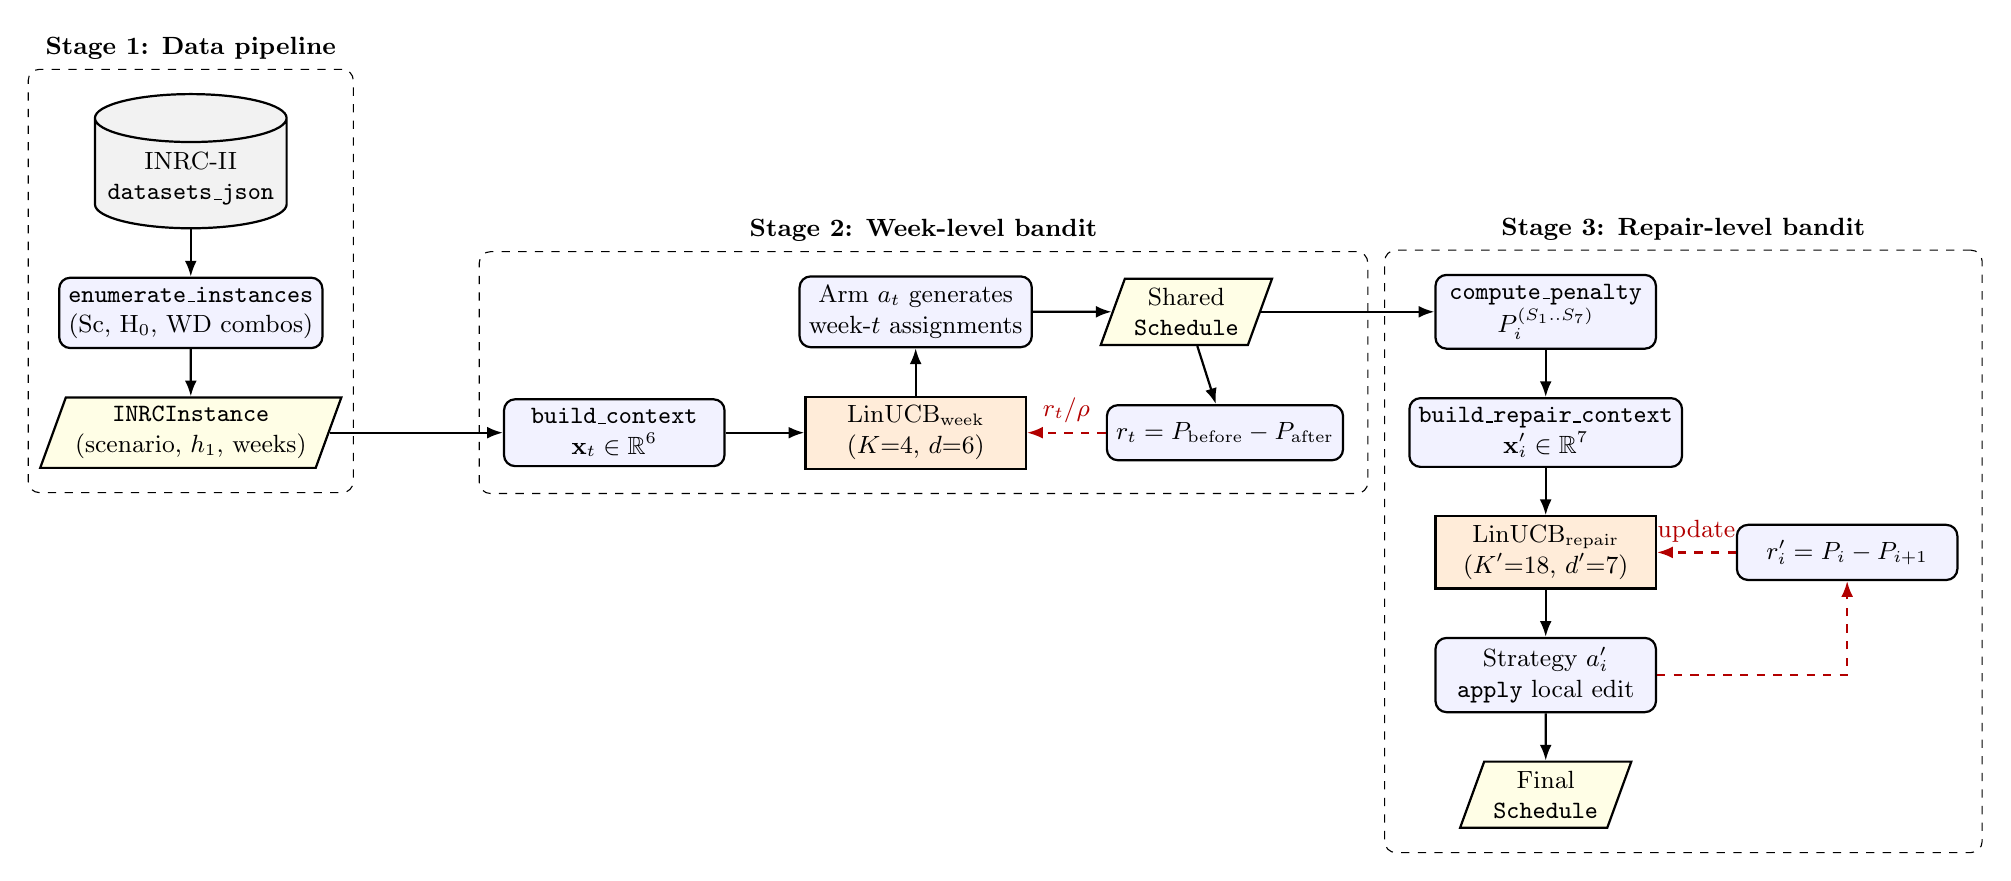
\begin{tikzpicture}[
  font=\small,
  node distance=6mm and 10mm,
  proc/.style   ={rectangle, rounded corners, draw, thick,
                  minimum width=28mm, minimum height=7mm,
                  align=center, fill=blue!5},
  data/.style   ={trapezium, trapezium left angle=70, trapezium right angle=110,
                  draw, thick, minimum width=20mm, align=center, fill=yellow!10},
  store/.style  ={cylinder, shape border rotate=90, aspect=0.25, draw, thick,
                  minimum height=12mm, minimum width=22mm,
                  align=center, text width=22mm, fill=gray!10},
  bandit/.style ={rectangle, draw, thick, minimum width=28mm, minimum height=9mm,
                  align=center, fill=orange!15},
  flow/.style   ={-{Latex[length=2mm]}, thick},
  reward/.style ={-{Latex[length=2mm]}, dashed, thick, red!70!black},
  stage/.style  ={draw, dashed, rounded corners, inner sep=3mm}
]

% ---------- Stage 1: vertical column ----------
\node[store] (ds) {INRC-II\\\texttt{datasets\_json}};
\node[proc, below=of ds]   (enum) {\texttt{enumerate\_instances}\\(Sc, H$_0$, WD combos)};
\node[data, below=of enum] (inst) {\texttt{INRCInstance}\\(scenario, $h_1$, weeks)};

% ---------- Stage 2: reward sits to the right of bandit ----------
\node[proc, right=22mm of inst] (ctx1) {\texttt{build\_context}\\$\mathbf{x}_t \in \mathbb{R}^{6}$};
\node[bandit, right=of ctx1]    (lin1) {LinUCB$_{\text{week}}$\\$(K{=}4,\,d{=}6)$};
\node[proc,   above=of lin1]    (arm1) {Arm $a_t$ generates\\week-$t$ assignments};
\node[data,   right=of arm1]    (sch1) {Shared\\\texttt{Schedule}};
\node[proc,   right=of lin1]    (pen1) {$r_t = P_{\text{before}} - P_{\text{after}}$};

% ---------- Stage 3: vertical chain, reward to the right of bandit ----------
\node[proc, right=22mm of sch1] (pen2)  {\texttt{compute\_penalty}\\$P_i^{(S_1..S_7)}$};
\node[proc,   below=of pen2]    (ctx2)  {\texttt{build\_repair\_context}\\$\mathbf{x}'_i \in \mathbb{R}^{7}$};
\node[bandit, below=of ctx2]    (lin2)  {LinUCB$_{\text{repair}}$\\$(K'{=}18,\,d'{=}7)$};
\node[proc,   below=of lin2]    (apply) {Strategy $a'_i$\\\texttt{apply} local edit};
\node[data,   below=of apply]   (out)   {Final\\\texttt{Schedule}};
\node[proc,   right=of lin2]    (rew2)  {$r'_i = P_i - P_{i+1}$};

% ---------- Arrows ----------
\draw[flow] (ds)          -- (enum);
\draw[flow] (enum)        -- (inst);
\draw[flow] (inst.east)   -- (ctx1.west);

\draw[flow]   (ctx1)      -- (lin1);
\draw[flow]   (lin1)      -- (arm1);
\draw[flow]   (arm1)      -- (sch1);
\draw[flow]   (sch1)      -- (pen1);
\draw[reward] (pen1)      -- node[above]{$r_t/\rho$} (lin1);

\draw[flow]   (sch1.east) -- (pen2.west);

\draw[flow]   (pen2)      -- (ctx2);
\draw[flow]   (ctx2)      -- (lin2);
\draw[flow]   (lin2)      -- (apply);
\draw[flow]   (apply)     -- (out);
\draw[reward] (apply.east) -| (rew2.south);
\draw[reward] (rew2)      -- node[above]{update} (lin2);

% ---------- Stage boxes ----------
\begin{scope}[on background layer]
  \node[stage, fit=(ds)(enum)(inst),
        label=above:\textbf{Stage 1: Data pipeline}] {};
  \node[stage, fit=(ctx1)(lin1)(arm1)(pen1)(sch1),
        label=above:\textbf{Stage 2: Week-level bandit}] {};
  \node[stage, fit=(pen2)(ctx2)(lin2)(apply)(out)(rew2),
        label=above:\textbf{Stage 3: Repair-level bandit}] {};
\end{scope}

\end{tikzpicture}}%
\caption{End-to-end pipeline. Stage~1 loads an INRC-II instance. Stage~2
runs the week-level LinUCB bandit: a 6-dim context $\mathbf{x}_t$ is
built from the instance, the bandit picks one of four construction
arms, and the resulting weekly schedule is appended to the shared
schedule. Stage~3 runs the repair-level LinUCB bandit for $N$ rounds:
a 7-dim context $\mathbf{x}'_i$ is built from the current
\texttt{PenaltyResult}, the bandit picks one of 18 repair strategies,
and the strategy mutates the shared schedule in place. Dashed red
arrows denote reward feedback $r = P_{\text{before}} - P_{\text{after}}$
fed to the corresponding bandit's ridge update.}
\label{fig:pipeline}
\end{figure}



\paragraph{Implementation Details.}
Both levels of the pipeline in Figure~\ref{fig:pipeline} are
implemented in Python on top of a NumPy disjoint-LinUCB backend.
The week-level bandit uses $K = 4$ construction arms
(\texttt{coverage\_first}, \texttt{fatigue\_aware},
\texttt{weekend\_balancing}, \texttt{preference\_respecting}) with a
$d = 6$ context; the repair-level bandit uses $K' = 18$
local-mutation arms grouped by target soft constraint with a
$d' = 7$ context. Unless stated otherwise we set the exploration
coefficient $\alpha = 1.0$, reward scale $\rho = 1000$ for the
week-level and $\rho = 50$ for the repair-level bandit, and run a
warm-start phase of round-robin arm selection for the first $R_w$
rounds before handing control back to LinUCB; this prevents a
cold-start collapse onto a single arm before the ridge matrices
accumulate enough signal to discriminate. Each experiment is
averaged over three random seeds $\{0, 1, 2\}$. Training state is
checkpointed as the per-arm $(\mathbf{A}_a, \mathbf{b}_a)$ pair in
\texttt{npz} format, accompanied by a JSON trajectory sidecar
recording the per-round reward, arm pick, and periodic $\theta$
snapshot for post-hoc diagnostics.

\paragraph{Datasets.}
We use the INRC-II benchmark~\cite{ceschia2015inrc2}, which
specifies instances through three kinds of JSON files: a scenario
file \texttt{Sc-*.json} fixing nurses, contracts, skills, and shift
types; a history file \texttt{H0-*.json} fixing the entry-state
$h_1$; and weekly demand files \texttt{WD-*.json} that define each
week's minimum and optimal coverage. An instance is assembled by
choosing one scenario, one history file, and an ordered tuple of
$W$ weekly-demand files. Our training stream is produced by
\texttt{enumerate\_instances}, which iterates all scenario families
(\texttt{n030w4}, \texttt{n060w4}, \texttt{n120w4}) across every
history file and samples up to
\texttt{week\_combos\_per\_scenario} week-tuples from the available
pool. Week-tuples are sampled \emph{without replacement} for the
main experiments and \emph{with replacement} for the larger
training runs in~\S\ref{subsec:training}; all combinatorial
enlargements are purely statistical sampling --- no dataset is
augmented with new solutions or labels, since the bandit training
loop is unsupervised.

\paragraph{Metrics.}
Since the bandit aims to minimize the INRC-II soft penalty
$P(\sigma, h)$ of the final schedule, our primary metric is
\emph{final penalty} at the end of the repair loop. We report it
alongside three complementary measures:
(i) the \emph{absolute penalty reduction}
$\Delta P = P_{\text{init}} - P_{\text{final}}$, which controls for
different per-instance baseline difficulty;
(ii) \emph{hard-violation counts} ($\text{H1}$--$\text{H4}$) of
the returned schedule, which must remain zero for the schedule to
be feasible at all; and
(iii) the \emph{rolling mean reward} over training, which
measures whether the bandit's per-round reward signal is improving
as it sees more instances. To diagnose the bandit itself we also
report the final arm-usage distribution and the L2 norm
$\|\theta_a\|_2$ per arm at periodic snapshots --- a flat norm
curve indicates the ridge estimate has saturated, which is the
empirical analogue of the confidence ellipsoid of
Lemma~\ref{lem:ellipsoid} having shrunk. Finally, we record
wall-clock \emph{runtime} (seconds) for the full pipeline (Stages
1--3 of Figure~\ref{fig:pipeline}) as a proxy for computational
efficiency, since the repair loop runs $N$ penalty evaluations per
instance and dominates cost for larger $|\mathcal{N}|$.

\begin{figure}[h]
    \centering 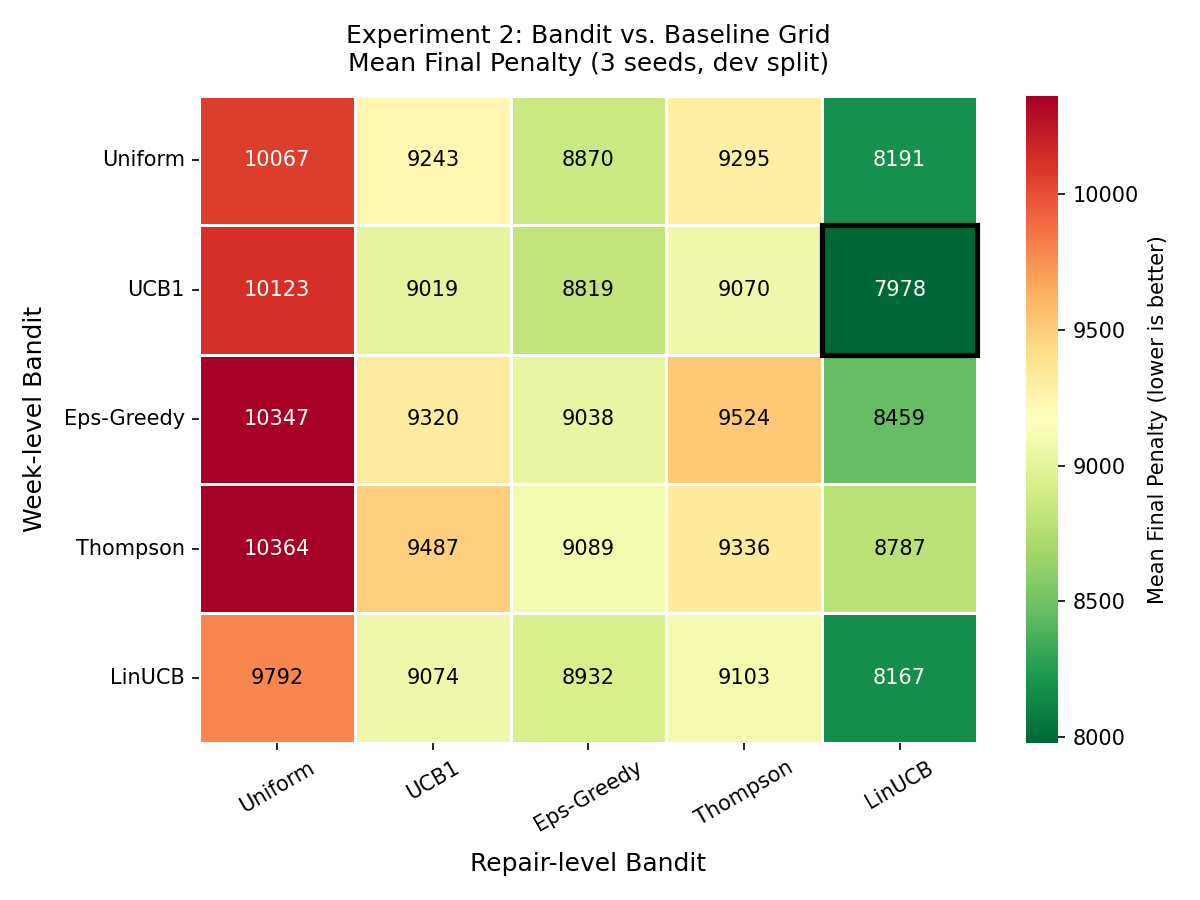
\includegraphics[width=0.55 \textwidth]{experiment plots/experiment-02/exp2_heatmap.png}
    \caption{Mean final penalty (averaged across 3 held-out sets and 3 random seeds) for every week-level $\times$ repair-level bandit pair. All 25 combinations of Uniform, UCB1, Epsilon-Greedy, Thompson Sampling, and LinUCB were evaluated. Week-level bandits picked from the 4 arms mentioned above, running the same number of rounds as the number of weeks in that scenario, while repair-level bandits chose from 18 constructed repair strategies over 500 rounds. The penalty at round 500 was recorded and averaged. The black border marks the best combination (\textsc{UCB1} $\times$ \textsc{LinUCB}, penalty $= 7{,}978$).}
    \label{fig:exp2_heatmap}
\end{figure}

\subsection{Training}\label{subsec:training}

% TODO: warm-start sweep, alpha sweep, reward-scale ablation,
%       with-replacement vs without.

\subsubsection{Sensitivity to LinUCB's exploration $\alpha$ parameter}
Upon investigating the sensitivity of final penalty to the exploration parameter $\alpha \in {0.25, 0.5, 1.0, 2.0}$, we trained a separate LinUCB model for each $\alpha$ value — fixing the seed, number 
of warm-up rounds, number of repair rounds, and number of training instances — sweeping independently for the week-level and repair-level bandits. $\alpha = 2.0$ achieved the lowest mean final penalty
and highest mean penalty reduction at both levels. However, the differences between this result and the other alphas is narrow, informing that performance is robust to $\alpha$ and no configuration is dramatically worse than another.


\begin{figure}[h]
    \centering 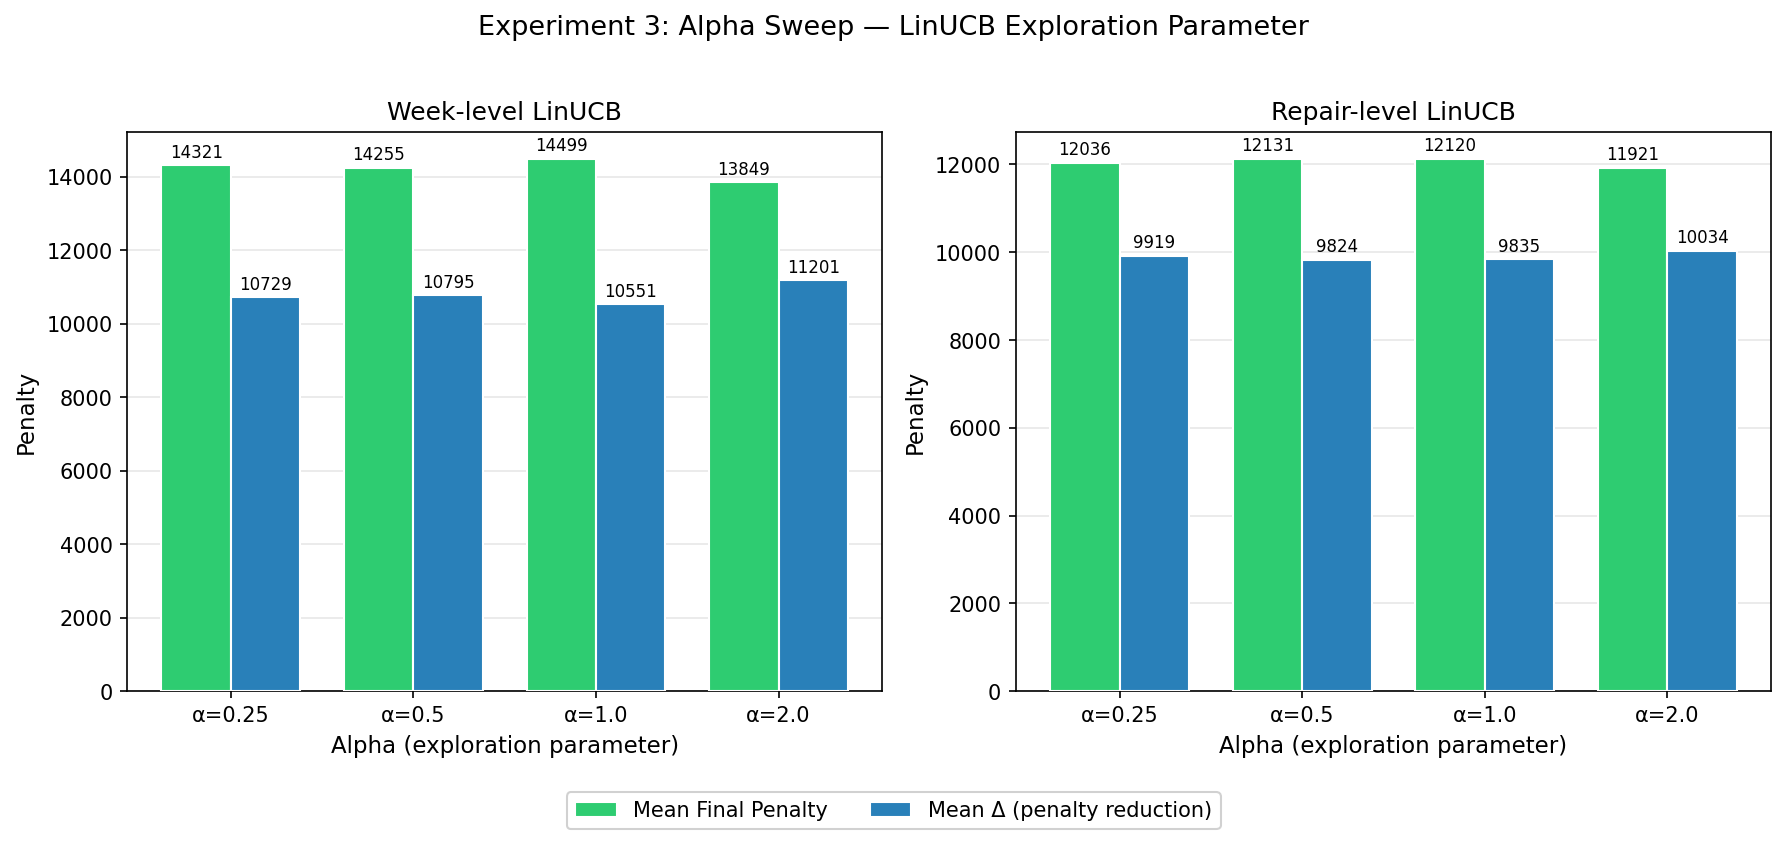
\includegraphics[width=0.55 \textwidth]{experiment plots/experiment-03/exp3_alpha_sweep.png}
    \caption{Mean final penalty and mean penalty reduction ($\Delta$) across four values of the LinUCB exploration parameter $\alpha \in \{0.25, 0.5, 1.0, 2.0\}$, evaluated on the held out scenarios. Results
   are shown separately for the week-level (left) and repair-level (right) bandits. $\alpha = 2.0$ achieves the lowest mean final penalty at both levels, indicating that higher exploration is beneficial  
  given the limited number of training instances.}
    \label{fig:exp3_alpha_sweep}
\end{figure}



\subsection{Comparing Contextual vs Non-Contextual Bandit Algorithm Performances }

% TODO: table comparing {uniform, ucb1, eps-greedy, linucb} at
%       week-level × {uniform, ucb1, linucb} at repair-level
%       on n030w4, n060w4, n120w4.

\begin{figure}[h]
    \centering 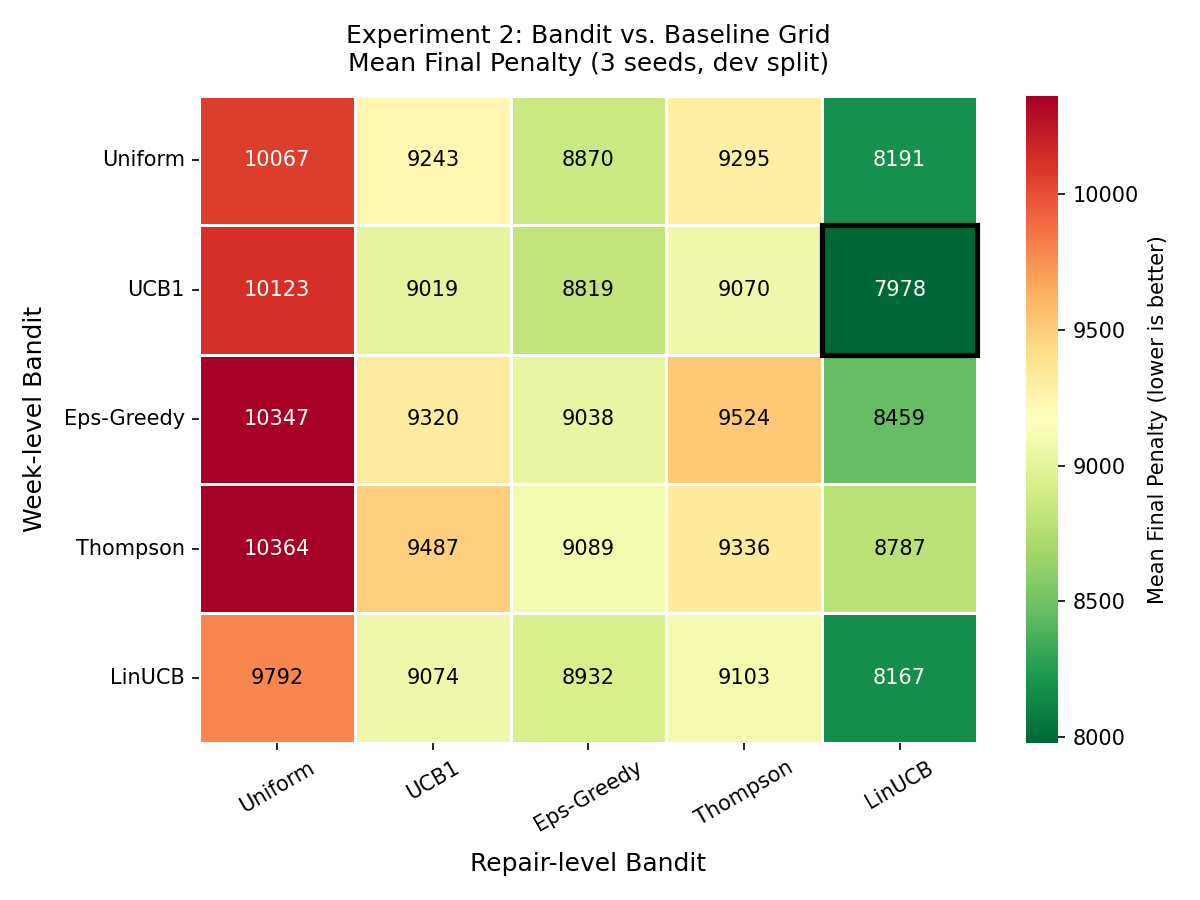
\includegraphics[width=0.55 \textwidth]{experiment plots/experiment-02/exp2_heatmap.png}
    \caption{Mean final penalty (averaged across 3 held-out sets and 3 random seeds) for every week-level $\times$ repair-level bandit pair. All 25 combinations of Uniform, UCB1, Epsilon-Greedy, Thompson Sampling, and LinUCB were evaluated. Week-level bandits picked from the 4 arms mentioned above, running the same number of rounds as the number of weeks in that scenario, while repair-level bandits chose from 18 constructed repair strategies over 500 rounds. The penalty at round 500 was recorded and averaged. The black border marks the best combination (\textsc{UCB1} $\times$ \textsc{LinUCB}, penalty $= 7{,}978$).}
    \label{fig:exp2_heatmap}
\end{figure}


As seen in Figure~\ref{fig:exp2_heatmap}, we see a clear pattern that despite any week-level bandit chosen to develop the pre-repaired schedule, choosing LinUCB as a repair-level bandit produced lower mean final penalties (with the rightmost column of the heatmap being shades of green). On the other hand, a Uniform repair-level bandit produces higher penalties across any week-level bandit. This is likely because LinUCB, as a contextual bandit, can leverage features of the current schedule state to select the most suitable repair strategy for each situation, whereas Uniform ignores this information and selects randomly. With 18 repair strategies available, random selection wastes many of the 500 rounds on inappropriate repairs, leading to slower convergence toward low-penalty schedules.

We also observe that the combination of the non-contextual UCB1 as the week-level and LinUCB as a repair-level bandit resulted in the lowest mean final penalty. While this opposes our initial hypothesis that the contextual LinUCB algorithms, as a week-level and repair-level bandit, would produce the lowest penalty, we observe that it produces the second-lowest penalty. A possible explanation is that at the week level, where only 4 arms are available and the number of arm selections per scenario is small (e.g., 8 times for an eight-week scenario), UCB1's confidence-bound-driven exploration is sufficient to identify the best arm without needing contextual information. Moroever, with such few arms and limited rounds, the context vectors that LinUCB relies on may introduce noise rather than useful signal.

A combination of either Thompson or $\epsilon$-Greedy as week-level and Uniform as repair-level produced the highest penalty, likely because stochastic exploration of these week-level methods occasionally commits to suboptimal weekly schedules, and without an intelligent repair-level policy to compensate causing the poor schedules are never effectively corrected and compounding errors at both stages.



\subsection{Diagnostics}

% TODO: drop in the four plots from scripts/plot_training.py:
%   reward_rolling.png, arm_usage_over_time.png,
%   theta_norms.png, final_theta_heatmap.png

\subsection{Model Performance as scenarios scale}

\begin{table}[h]
\centering
\begin{tabular}{llccc}                                                                                                          
\toprule
\textbf{Split} & \textbf{Scenarios} & \textbf{$n$} & \textbf{Mean Final Penalty} & \textbf{Mean $\Delta$} \\                                                                                              
\midrule                                                                                                                      
Dev  & n005w4, n012w8, n021w4       & 9  & 10,590 & 3,259  \\
Val  & n035--n110, w4/w8            & 10 & 60,214 & 14,933 \\ 
Test & n030--n120, w4/w8/w16/w32    & 10 & 96,945 & 18,192 \\
\bottomrule                                                           \end{tabular}          

\caption{Experiment 7: Cross-split generalization of the best LinUCB checkpoint (week $\alpha=2.0$, repair $\alpha=2.0$, 500 repair rounds). Mean final penalty and mean penalty reduction ($\Delta$) are 
reported per split. The increase in absolute penalty from dev to test reflects the larger scenario sizes rather than performance degradation; the mild decline in relative reduction (dev: 23.5\%, val:   
19.9\%, test: 15.8\%) indicates a degree of domain shift when generalizing to unseen scenario sizes and week horizons.}
\label{tab:exp7_generalization}                                                                                                                                                                     
\end{table}
\subsubsection{Arm usage over time}

\subsubsection{theta_norms}


% TODO: describe n030w4 dataset, episode structure,
%       alpha sweep, comparison with random arm selection


% ============================================================
\section{Open Problems and Future Directions}
% ============================================================

% TODO

\appendix

\section{Notation from the INRC-II Mathematical Model}
\label{app:notation}

The following notation is drawn directly from the INRC-II mathematical
model specification ~\cite{ceschia2015inrc2}. It is reproduced here for
reference since the model document is cited but not included in this
report.

\subsection*{Sets}

\begin{tabular}{@{}lp{10cm}@{}}
  $\mathcal{N}$ &
    Set of nurses. $|\mathcal{N}|$ denotes the total number of
    nurses in the scheduling instance. \\[6pt]

  $\mathcal{D}$ &
    Set of days in the planning horizon. $|\mathcal{D}|$ denotes the
    total number of days; a single week has $|\mathcal{D}| = 7$. \\[6pt]

  $\mathcal{S}$ &
    Set of shift types (e.g.\ Early, Late, Night). $|\mathcal{S}|$
    denotes the number of distinct shift types. Day-off is not
    counted as a shift type. \\[6pt]

  $\mathcal{SK}$ &
    Set of skills. Nurses may hold one or more skills (e.g.\
    Head Nurse, Nurse, Caregiver). \\[6pt]

  $\mathcal{W}$ &
    Set of weekends in the planning horizon. Each weekend consists of
    exactly two consecutive days (Saturday and Sunday), so
    $|\mathcal{W}| = \lfloor |\mathcal{D}| / 7 \rfloor$. \\[6pt]

  $F$ &
    Set of forbidden shift-type successions. Each element $f \in F$
    is a pair $(s_1, s_2)$ meaning shift $s_2$ may not follow shift
    $s_1$ on consecutive days. \\[6pt]

  $\mathcal{SK}_n$ &
    Set of skills held by nurse $n$. \\
\end{tabular}

\subsection*{Decision variables}

\begin{tabular}{@{}lp{10cm}@{}}
  $x_{n,d,s,sk} \in \{0,1\}$ &
    Equal to $1$ if nurse $n$ is assigned shift type $s$ requiring
    skill $sk$ on day $d$; $0$ otherwise. \\[6pt]

  $o_{n,d,s} \in \{0,1\}$ &
    Equal to $1$ if nurse $n$ works shift $s$ on day $d$ under any
    skill; $0$ otherwise. Defined as
    $o_{n,d,s} = \sum_{sk \in \mathcal{SK}} x_{n,d,s,sk}$. \\[6pt]

  $p_{n,d} \in \{0,1\}$ &
    Equal to $1$ if nurse $n$ works any shift on day $d$; $0$
    otherwise. Defined as $p_{n,d} = \sum_{s \in \mathcal{S}}
    o_{n,d,s}$. \\[6pt]

  $q_{n,w} \in \{0,1\}$ &
    Equal to $1$ if nurse $n$ works any shift during weekend $w$;
    $0$ otherwise. \\
\end{tabular}

\subsection*{Problem parameters}

\begin{tabular}{@{}lp{10cm}@{}}
  $C^{\min}_{d,s,sk}$ &
    Hard minimum number of nurses with skill $sk$ required to cover
    shift $s$ on day $d$. Enforced by hard constraint H2. \\[6pt]

  $C^{\text{opt}}_{d,s,sk}$ &
    Soft optimal number of nurses with skill $sk$ that should be
    assigned shift $s$ on day $d$. Falling below this target
    incurs a penalty under S1. \\[6pt]

  $C^{\text{opt}}_{\max}$ &
    Shorthand for $\max_{d,s,sk}\, C^{\text{opt}}_{d,s,sk}$, the
    largest optimal staffing requirement across all
    day--shift--skill combinations. \\[6pt]

  $CW^{\min}_n,\, CW^{\max}_n$ &
    Minimum and maximum number of consecutive working days allowed
    for nurse $n$ under their contract. Soft constraint S2. \\[6pt]

  $CF^{\min}_n,\, CF^{\max}_n$ &
    Minimum and maximum number of consecutive days off allowed for
    nurse $n$ under their contract. Soft constraint S3. \\[6pt]

  $CW_n \in \{0,1\}$ &
    Contract flag equal to $1$ if nurse $n$ is required to work
    complete weekends (both Saturday and Sunday, or neither); $0$
    if partial weekends are permitted. Soft constraint S5. \\[6pt]

  $T^{\min}_n,\, T^{\max}_n$ &
    Minimum and maximum total number of shifts nurse $n$ should work
    over the full planning horizon. Soft constraint S6. \\[6pt]

  $TW^{\max}_n$ &
    Maximum total number of weekends nurse $n$ may work over the
    full planning horizon. Soft constraint S7. \\
\end{tabular}

\subsection*{History variables}

These values are carried over from the previous planning horizon and
form part of the history $h$ passed to $P(\sigma, h)$.

\begin{tabular}{@{}lp{10cm}@{}}
  $h^{CW}_n$ &
    Number of consecutive working days nurse $n$ had at the end of
    the previous planning horizon. Used to initialise the working-run
    count at the start of the current week (S2). Equal to $0$ if the
    nurse had at least one day off at the end of the previous
    horizon. \\[6pt]

  $h^{CF}_n$ &
    Number of consecutive days off nurse $n$ had at the end of the
    previous planning horizon. Used to initialise the rest-run count
    at the start of the current week (S3). Equal to $0$ if the nurse
    was working at the end of the previous horizon. \\
\end{tabular}

\subsection*{Request sets}

\begin{tabular}{@{}lp{10cm}@{}}
  $\mathit{SOR}$ &
    Set of shift-off requests. Each element is a tuple $(n, d, s)$
    representing nurse $n$'s request not to be assigned shift $s$ on
    day $d$. Soft constraint S4. \\[6pt]

  $\mathit{DOR}$ &
    Set of day-off requests. Each element is a tuple $(n, d)$
    representing nurse $n$'s request for the entire day $d$ off.
    Soft constraint S4. \\
\end{tabular}

\subsubsection{Range/bounds of each component}
Each component of $P(\sigma, h)$ counts how many times an undesirable
event occurs in the schedule. The notation used throughout this section
follows the INRC-II mathematical model~\cite{ceschia2015inrc2}; a
complete reference list of symbols is given in
Appendix~\ref{app:notation}. For each component we derive a worst-case
upper bound by replacing every term in the sum by its maximum possible
value and multiplying by the number of terms.

\paragraph{S1 -- Coverage $P_{\text{cov}}$}

For each nurse $n$, each day $d$, and each shift type $s$, this
component measures how far the nurse's contribution falls short of the
optimal staffing target $C^{\text{opt}}_{d,s,sk}$. Overstaffing is not
penalised. Since $x_{n,d,s,sk} \in \{0,1\}$, the worst case for a
single triple $(n,d,s)$ is $x_{n,d,s,sk} = 0$, giving a shortfall of
$C^{\text{opt}}_{d,s,sk} \leq C^{\text{opt}}_{\max}$. The sum ranges
over $|\mathcal{N}| \times |\mathcal{D}| \times |\mathcal{S}|$ such
triples, so:
\[
  P_{\text{cov}}
  \;\leq\;
  |\mathcal{N}|\,|\mathcal{D}|\,|\mathcal{S}|\,C^{\text{opt}}_{\max}.
\]
Hard constraint H2 guarantees the hard minimum staffing $C^{\min}$ is
always met structurally, so $P_{\text{cov}}$ only fires for shortfalls
below the \emph{soft} optimal target, not catastrophic understaffing.
It does not depend on history $h$ since coverage is evaluated entirely
within the current week.

\paragraph{S2 -- Consecutive working days $P_{\text{consec}}$}

Each nurse $n$ has contract bounds $[CW^{\min}_n, CW^{\max}_n]$ on the
length of any contiguous block of working days. A block longer than
$CW^{\max}_n$ contributes its excess length; a block shorter than
$CW^{\min}_n$ contributes its deficit. In the worst case a nurse
alternates between working and resting every single day across the
horizon, maximising the number of one-day working blocks each of which
is shorter than $CW^{\min}_n$. The total violation for one nurse is
therefore at most $|\mathcal{D}|$, and summing over all
$|\mathcal{N}|$ nurses gives:
\[
  P_{\text{consec}} \;\leq\; |\mathcal{N}|\,|\mathcal{D}|.
\]
History $h$ is required because a working block may have started in a
prior week; $h^{CW}_n$ records the number of consecutive working days
at the end of the previous horizon so that the block length is counted
correctly at the start of the current week.

\paragraph{S3 -- Consecutive days off $P_{\text{off}}$}

Each nurse $n$ has contract bounds $[CF^{\min}_n, CF^{\max}_n]$ on the
length of any contiguous rest block. By the same alternating argument
as S2, the worst case produces the maximum number of one-day rest
blocks across the horizon, giving a total violation of at most
$|\mathcal{D}|$ per nurse. Summing over all $|\mathcal{N}|$ nurses:
\[
  P_{\text{off}} \;\leq\; |\mathcal{N}|\,|\mathcal{D}|.
\]
History $h$ is required via $h^{CF}_n$, the number of consecutive rest
days carried over from the previous horizon, for the same
initialisation reason as S2.

\paragraph{S4 -- Preferences $P_{\text{pref}}$}

Nurses submit shift-off requests $\mathit{SOR}$ and day-off requests
$\mathit{DOR}$; each ignored request contributes exactly one violation.
For a single nurse--day pair $(n,d)$, the contribution is at most $1$
(the request is either ignored or honoured). The sum ranges over at
most $|\mathcal{N}| \times |\mathcal{D}|$ such pairs, so:
\[
  P_{\text{pref}} \;\leq\; |\mathcal{N}|\,|\mathcal{D}|.
\]
Preferences are local to the current week and do not depend on
history $h$.

\paragraph{S5 -- Complete weekends $P_{\text{wknd}}$}

For nurses with $CW_n = 1$, working exactly one day of a weekend
(Saturday or Sunday but not both) contributes one violation; working
both or neither does not. For a single nurse--weekend pair $(n,w)$,
the contribution is therefore at most $1$. There are
$|\mathcal{N}| \times |\mathcal{W}|$ such pairs, where
$|\mathcal{W}| = \lfloor |\mathcal{D}|/7 \rfloor$, giving:
\[
  P_{\text{wknd}}
  \;\leq\;
  |\mathcal{N}|\,|\mathcal{W}|
  \;=\;
  |\mathcal{N}|\!\left\lfloor\frac{|\mathcal{D}|}{7}\right\rfloor.
\]
This bound is strictly tighter than $|\mathcal{N}||\mathcal{D}|$ since
$|\mathcal{W}| \ll |\mathcal{D}|$; for a 28-day horizon
$|\mathcal{W}| = 4$ versus $|\mathcal{D}| = 28$. History $h$ is
needed to track weekends already worked in prior weeks.

\paragraph{S6 -- Total assignments $P_{\text{total}}$}

Each nurse $n$ has a contract interval $[T^{\min}_n, T^{\max}_n]$ for
the total number of shifts worked over the full planning horizon. The
violation counts how far outside this interval the nurse's cumulative
total falls. Since hard constraint H1 enforces at most one shift per
day, the total for any nurse is bounded by $|\mathcal{D}|$, so the
excess above $T^{\max}_n$ or the deficit below $T^{\min}_n$ is at most
$|\mathcal{D}|$ per nurse. Summing over all $|\mathcal{N}|$ nurses:
\[
  P_{\text{total}} \;\leq\; |\mathcal{N}|\,|\mathcal{D}|.
\]
History $h$ is required because $T^{\min}_n$ and $T^{\max}_n$ are
cumulative over the full horizon; shifts worked in prior weeks
contribute to the running total.

\paragraph{S7 -- Total working weekends $P_{\text{wkndmax}}$}

Each nurse $n$ has a contract maximum $TW^{\max}_n$ on the total
number of weekends worked over the full horizon. The violation counts
how many weekends exceed this limit. Since the total number of weekends
any nurse can work is at most $|\mathcal{W}|$, the excess above
$TW^{\max}_n$ is at most $|\mathcal{W}|$ per nurse. Summing over all
$|\mathcal{N}|$ nurses:
\[
  P_{\text{wkndmax}}
  \;\leq\;
  |\mathcal{N}|\,|\mathcal{W}|
  \;=\;
  |\mathcal{N}|\!\left\lfloor\frac{|\mathcal{D}|}{7}\right\rfloor.
\]
History $h$ is required to track weekends already worked before the
current planning week, for the same cumulative reason as S6.

\paragraph{Combined bound}

Substituting all seven components into $P(\sigma, h)$ and applying the
INRC-II weights $(w_1,\ldots,w_7) = (30,\,15/30,\,30,\,10,\,30,\,20,
\,30)$~\cite{ceschia2015inrc2}:
\begin{align}
  P(\sigma, h)
  \;\leq\;&\;
  w_1\,|\mathcal{N}|\,|\mathcal{D}|\,|\mathcal{S}|\,C^{\text{opt}}_{\max}
  \;+\;
  (w_2 + w_3 + w_4 + w_6)\,|\mathcal{N}|\,|\mathcal{D}|
  \notag\\[4pt]
  &+\;
  (w_5 + w_7)\,|\mathcal{N}|
  \!\left\lfloor\frac{|\mathcal{D}|}{7}\right\rfloor
  \;=:\; R_{\max}.
  \label{eq:rmax}
\end{align}
Since every component is a sum of non-negative violation counts,
$P(\sigma, h) \geq 0$ for any schedule $\sigma$ and history $h$.
Both $\sigma_t^{\text{before}}$ and $\sigma_t^{\text{after}}$ are
valid schedules over the same finite problem instance and therefore
satisfy $P \in [0, R_{\max}]$, which gives
$r_t \in [-R_{\max}, R_{\max}]$ as required by
Proposition~\ref{prop:bounded}.

\bibliographystyle{plainnat}
\begin{thebibliography}{9}

\bibitem{chu2011contextual}
Chu, W., Li, L., Reyzin, L., \& Schapire, R.~E. (2011).
\textit{Contextual bandits with linear payoff functions}.
In \textit{Proceedings of AISTATS}, pp.~208--214.

\bibitem{abbasi2011improved}
Abbasi-Yadkori, Y., P{\'a}l, D., \& Szepesv{\'a}ri, C. (2011).
\textit{Improved algorithms for linear stochastic bandits}.
In \textit{Advances in Neural Information Processing Systems (NeurIPS)}.

\bibitem{li2010contextual}
Li, L., Chu, W., Langford, J., \& Schapire, R.~E. (2010).
\textit{A contextual-bandit approach to personalized news article recommendation}.

\bibitem{ceschia2015inrc2}
Ceschia, S., Dang, N.~T.~T., De Causmaecker, P., Haspeslagh, S.,
\& Schaerf, A. (2019).
\textit{The Second International Nurse Rostering Competition}.
\textit{Annals of Operations Research}, 274(1--2), 171--186.


In \textit{Proceedings of WWW}, pp.~661--670.


% TODO: add INRC-II competition paper (Sc\"onberger et al. 2016)
% TODO: add nurse rostering survey

\end{thebibliography}

\end{document}



-------------------------------------
\subsection{Comparing Contextual vs Non-Contextual Bandit Algorithm Performances } %Experiment - 02

\begin{figure}[h]
    \centering 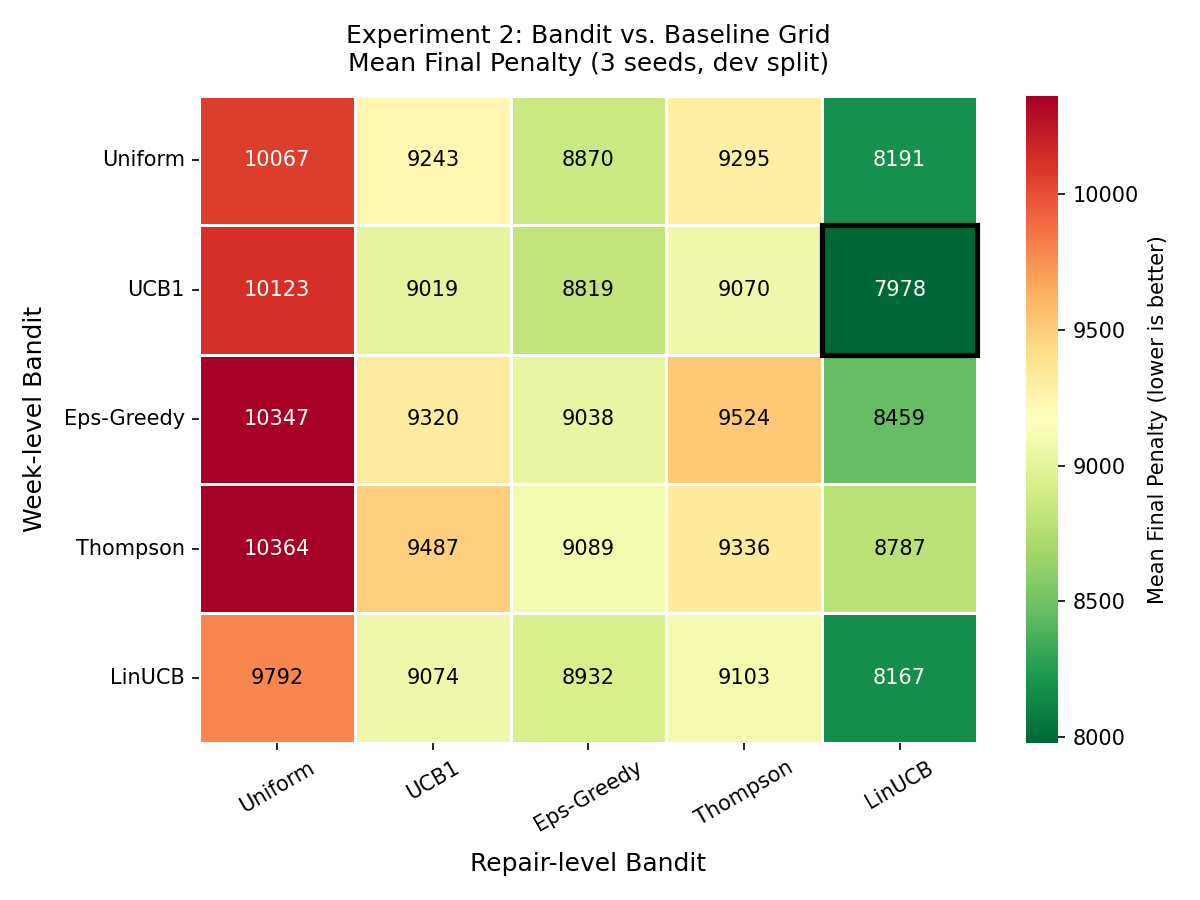
\includegraphics[width=0.5\textwidth]{experiment plots/experiment-02/exp2_heatmap.png}
    \caption{Mean final penalty (averaged across 3 held-out sets and 3 random seeds) for every week-level $\times$ repair-level bandit pair. All 25 combinations of Uniform, UCB1, Epsilon-Greedy, Thompson Sampling, and LinUCB were evaluated. Week-level bandits picked from the 4 arms mentioned above, running the same number of rounds as the number of weeks in that scenario, while repair-level bandits chose from 18 constructed repair strategies over 500 rounds. The penalty at round 500 was recorded and averaged. The black border marks the best combination (\textsc{UCB1} $\times$ \textsc{LinUCB}, penalty $= 7{,}978$).}
    \label{fig:exp2_heatmap}
\end{figure}

In Figure~\ref{fig:exp2_heatmap}, we see a clear pattern that despite any week-level bandit chosen to develop the pre-repaired schedule, choosing LinUCB as a repair-level bandit produced lower mean final penalties -with the rightmost column of the heatmap being shades of green. On the other hand, a Uniform repair-level bandit produces higher penalties across any week-level bandit. This is likely because with 18 repair strategies available, uniform selection wastes many of the 500 rounds on inappropriate repairs, leading to slower convergence toward low-penalty schedules. 

LinUCB also performs better than UCB1, $\epsilon$- Greedy, Thompson sampling. This could possibly be since these three algorithms learn and choose an arm that looked best on average, regardless of whether in the current schedule context, 
is coverage-dominated or fatigue-dominated.
single global ranking over the 18 operators

We also observe that the combination of the non-contextual UCB1 as the week-level and LinUCB as a repair-level bandit resulted in the lowest mean final penalty. While this opposes our initial hypothesis that the contextual LinUCB algorithms, as a week-level and repair-level bandit, would produce the lowest penalty, we observe that it produces the second-lowest penalty. A possible explanation is that at the week level, where only 4 arms are available and the number of arm selections per scenario is small (e.g., 8 times for an eight-week scenario), UCB1's confidence-bound-driven exploration is sufficient to identify the best arm without needing contextual information. Moroever, with such few arms and limited rounds, the context vectors that LinUCB relies on may introduce noise rather than useful signal.

A combination of either Thompson or $\epsilon$-Greedy as week-level and Uniform as repair-level produced the highest penalty, likely because stochastic exploration of these week-level methods occasionally commits to suboptimal weekly schedules, and without an intelligent repair-level policy to compensate causing the poor schedules are never effectively corrected and compounding errors at both stages.

% 1. Per-arm selection frequency analysis. You have 4 construction arms and 18 repair arms. Showing which arms LinUCB selects across different contexts would directly demonstrate that the contextual policy is doing something meaningful — not just converging to one dominant arm. A heatmap of arm-selection frequency vs. context regime (e.g., coverage-dominated vs. fatigue-dominated weeks) would be very informative.


% 2. Cumulative regret curves. You discuss regret bounds theoretically but never show empirical regret. Plotting cumulative reward of LinUCB vs. the oracle best-fixed-arm (or best-context-dependent-arm) would quantify how much the bandit is actually learning over time, and how fast.

\subsection{Cumulative Reward of Adaptive vs. Fixed-Arm Policies at the Week-Level Construction Stage}

\label{sec:warm-start}
\begin{figure}[h] 
    \centering
    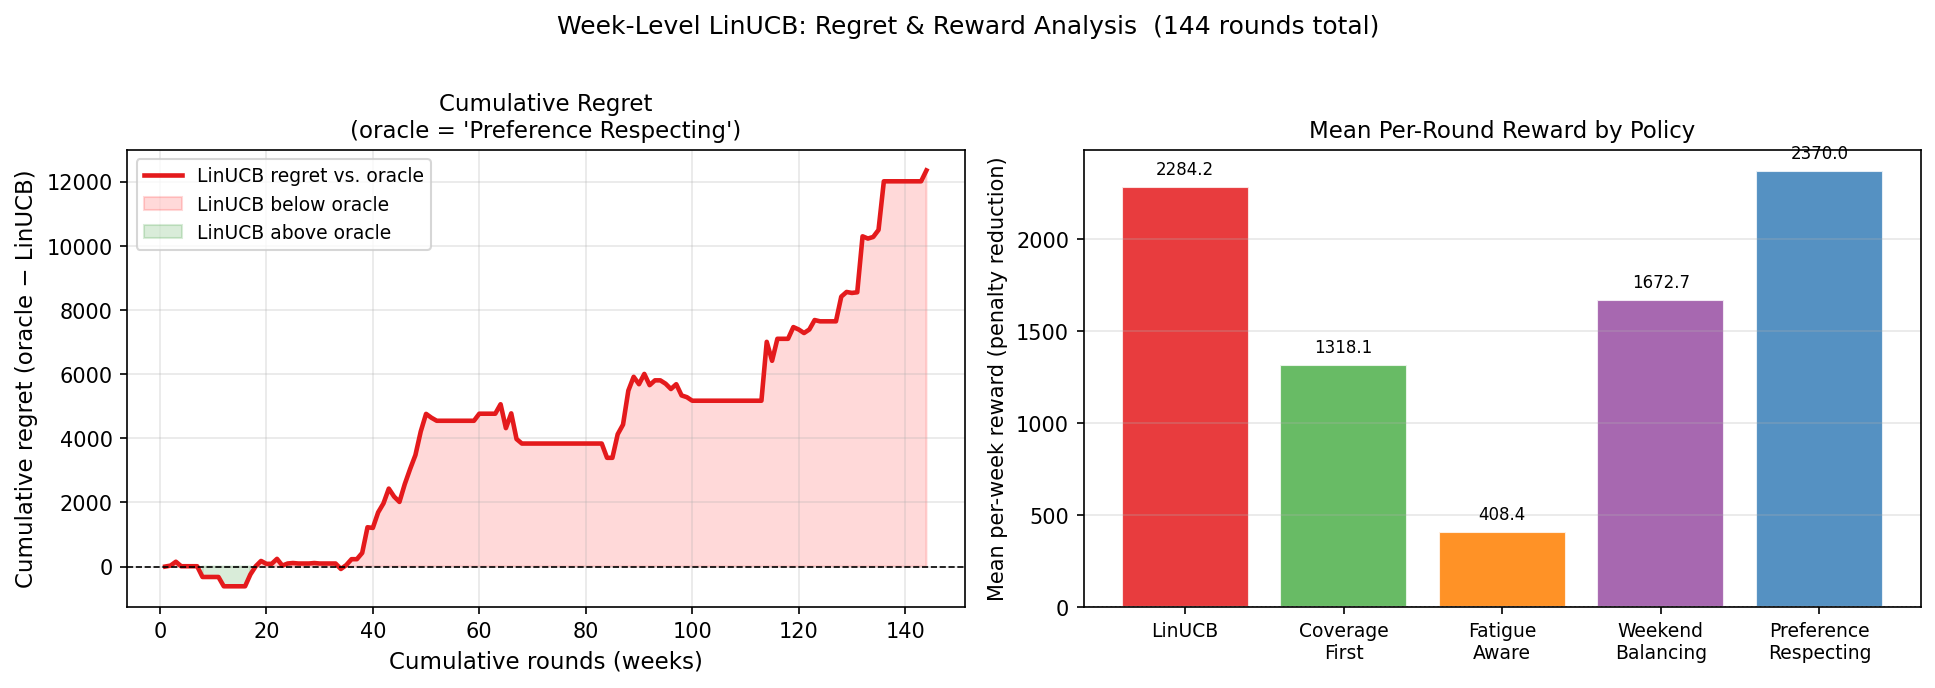
\includegraphics[width=0.48\textwidth]{experiment plots/exp: adaptive vs fixed cumilative/cumulative_regret.png}
    \hfill
    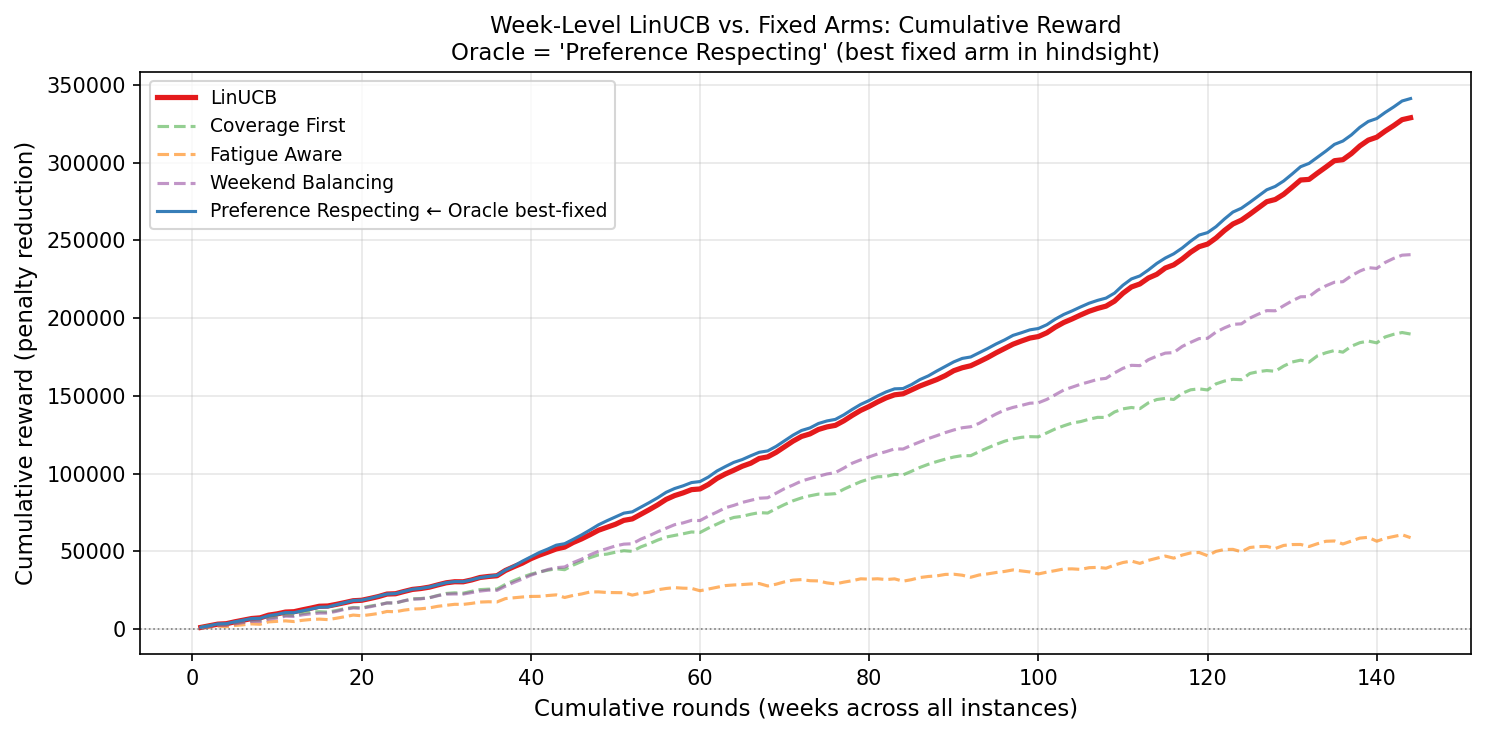
\includegraphics[width=0.48\textwidth]{experiment plots/exp: adaptive vs fixed cumilative/cumulative_reward.png}
    \caption{..}
    \label{fig:warm-start}
\end{figure}

\subsection{Parameter Sensitivity Studies}
\subsubsection{LinUCB's exploration $\alpha$ parameter}

\begin{figure}[h]
    \centering 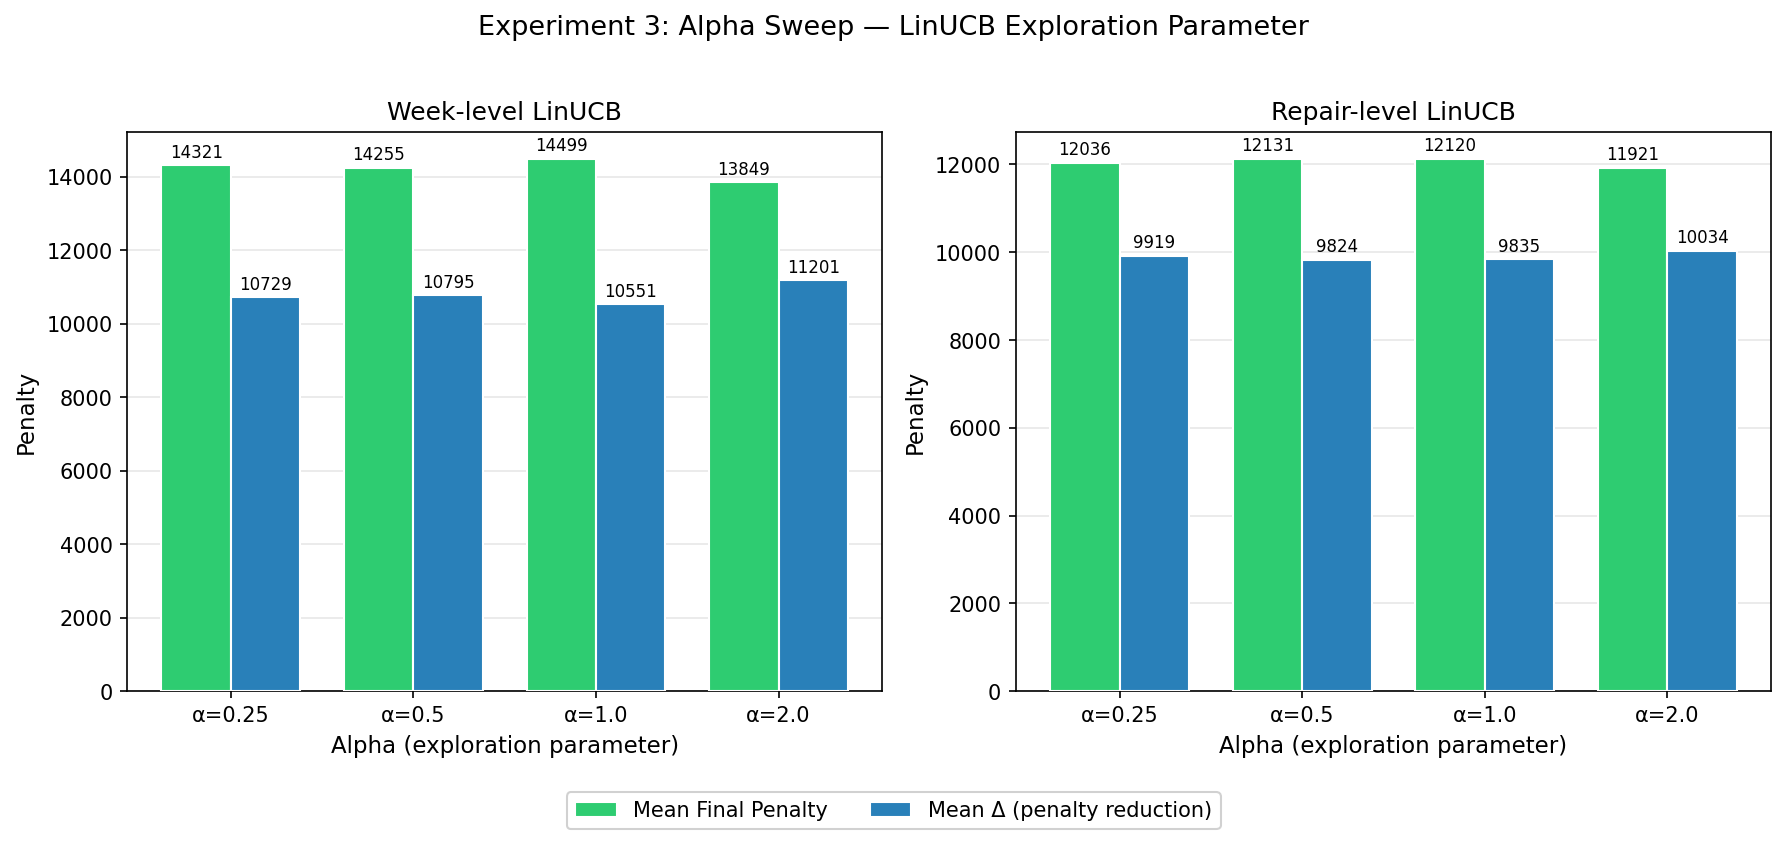
\includegraphics[width=0.55 \textwidth]{experiment plots/experiment-03/exp3_alpha_sweep.png}
    \caption{Mean final penalty and mean $\Delta$ across $\alpha \in {0.25, 0.5, 1.0, 2.0}$ for the week-level (left) and repair-level (right) LinUCB bandits, evaluated on held-out scenarios. $\alpha = 2.0$ achieves
   the lowest final penalty at both levels.}
    \label{fig:exp3_alpha_sweep}
\end{figure}

Upon investigating the sensitivity of final penalty to the exploration parameter $\alpha \in {0.25, 0.5, 1.0, 2.0}$, we trained a separate LinUCB model for each $\alpha$ value — fixing the seed, number 
of warm-up rounds, number of repair rounds, and number of training instances — sweeping independently for the week-level and repair-level bandits. As seen in Figure~\ref{fig:exp3_alpha_sweep}, $\alpha = 2.0$ achieved the lowest mean final penalty
and highest mean penalty reduction at both levels. However, the differences between this result and the other alphas is narrow, informing that performance is robust to $\alpha$ and no configuration is dramatically worse than another.

\subsubsection{Reward-scale sensitivity} % Experiment - 04 
\begin{figure}[h]
    \centering
    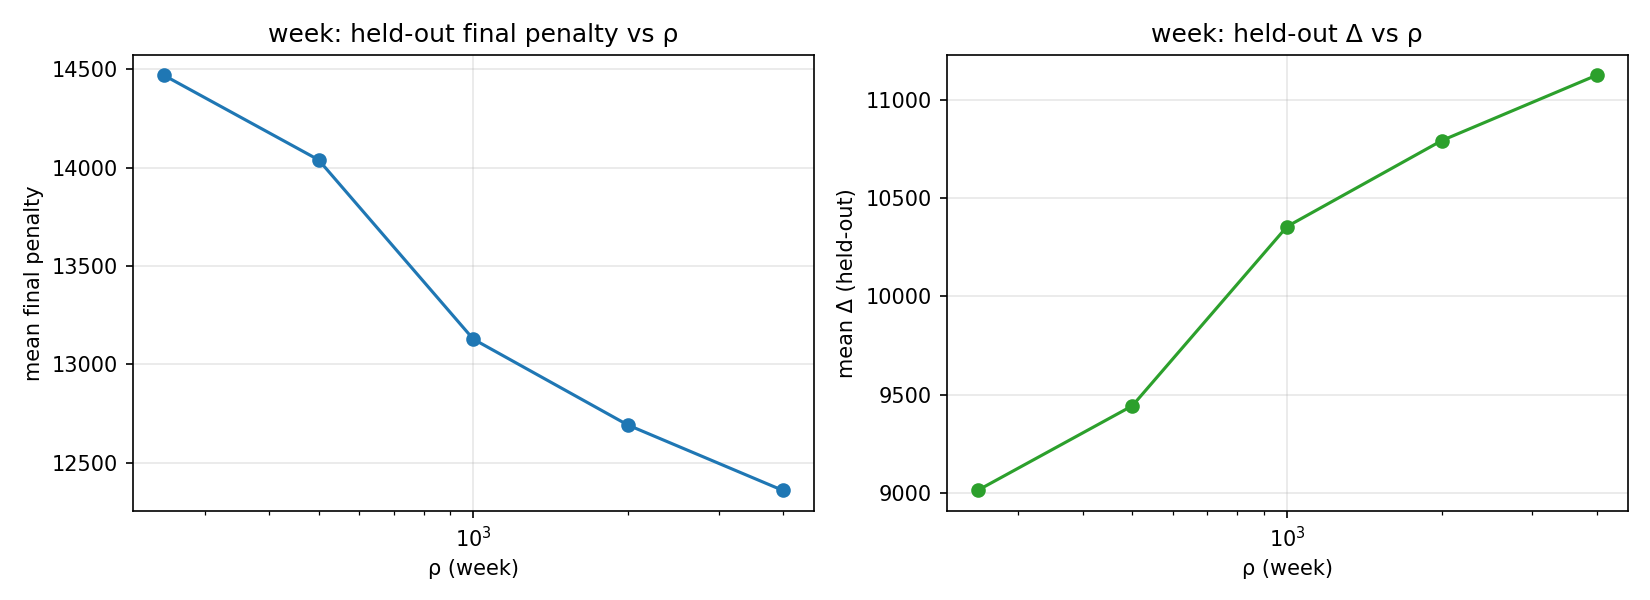
\includegraphics[width=0.48\textwidth]{experiment plots/experiment-04/reward_scale_week.png}
    \hfill
    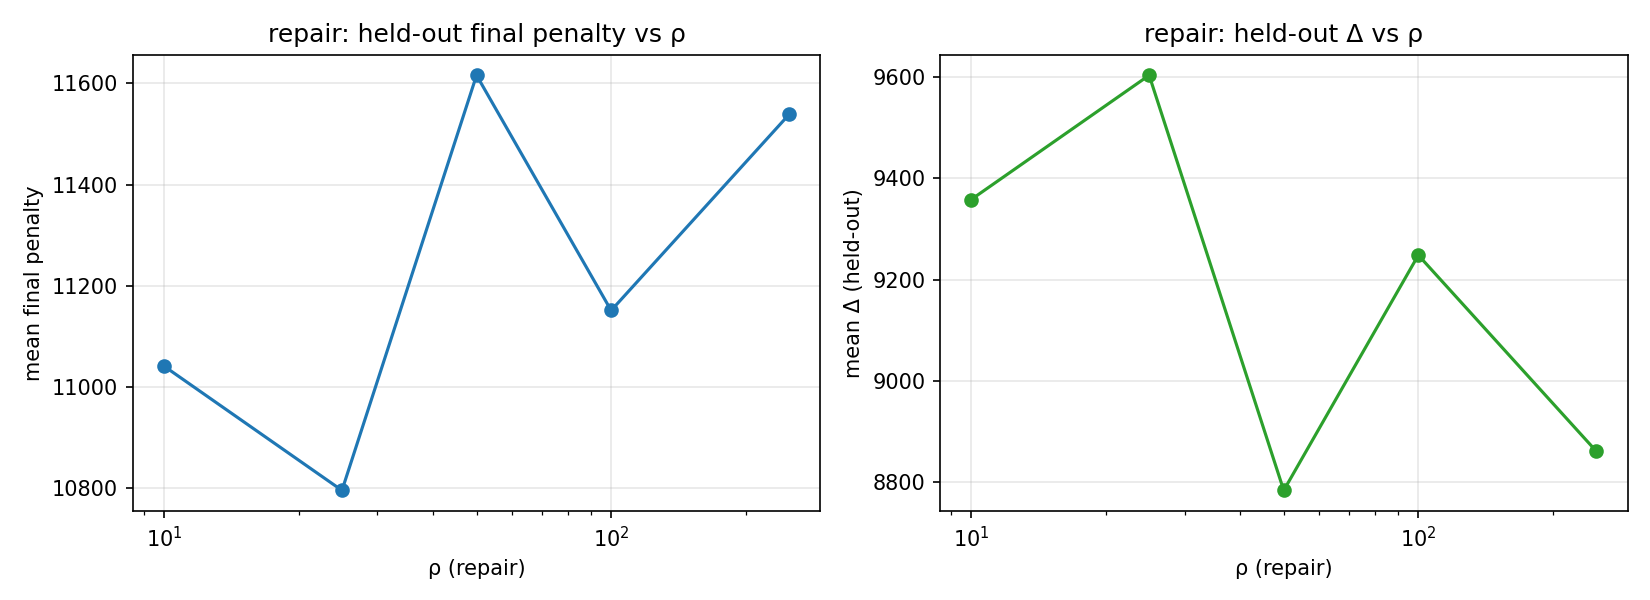
\includegraphics[width=0.48\textwidth]{experiment plots/experiment-04/reward_scale_repair.png}
    \caption{Held-out dev mean final penalty and mean $\Delta$ vs.\ reward scale $\rho$ at the week level (left) and repair level (right).}
    \label{fig:reward-scale}
\end{figure}

The reward-scale parameter $\rho$ normalises raw penalty deltas before they enter the bandit update: $r = \Delta P / \rho$. At the week level, mean final penalty decreases monotonically as $\rho$ increases.At the repair level, performance is erratic across $\rho$ values. Larger $\rho$ compresses reward magnitudes toward zero, which slows the
growth of the estimated coefficients $\hat{\theta}_a$ relative to the
exploration bonus $\alpha\sqrt{\mathbf{x}^\top A_a^{-1}\mathbf{x}}$,
effectively prolonging exploration, which sees to be favorable when the arm
space is small and the cost of trying each arm is low.  

\subsection{Warm-start length} % Experiment - 05
\label{sec:warm-start}
\begin{figure}[h] 
    \centering
    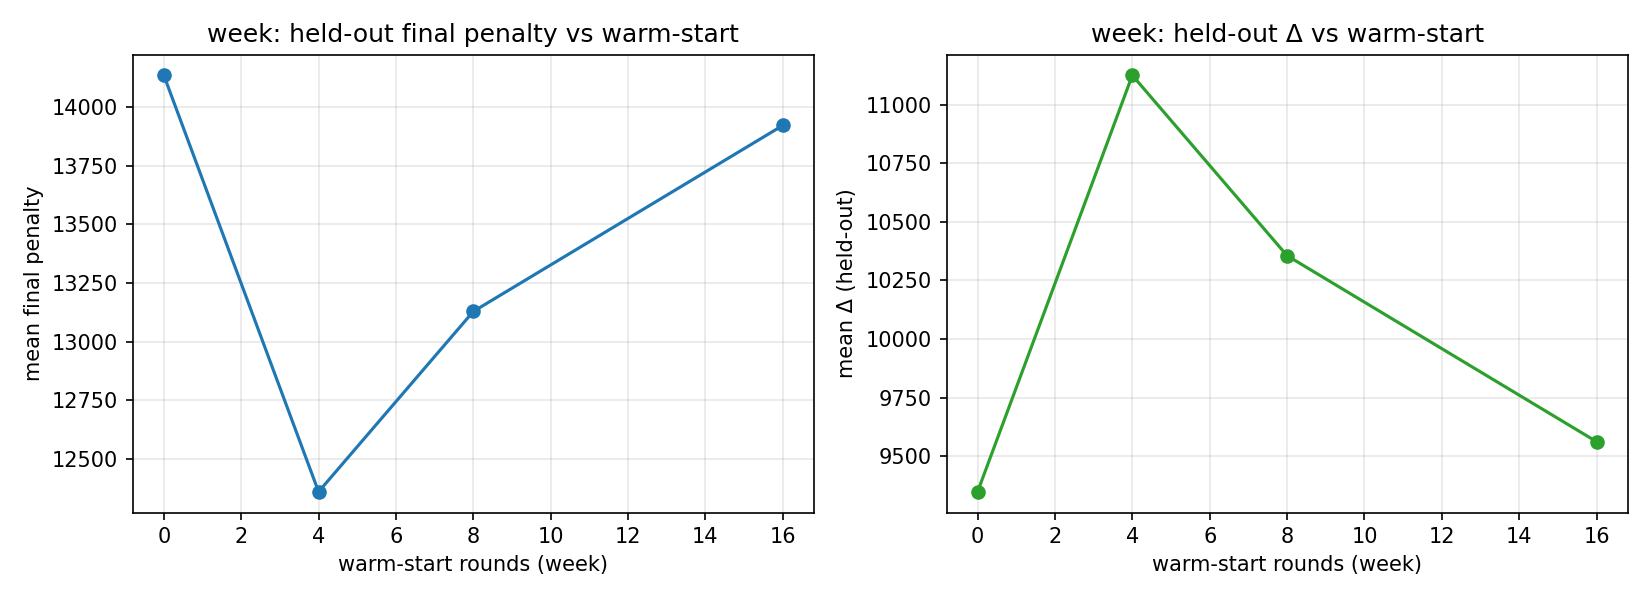
\includegraphics[width=0.48\textwidth]{experiment plots/experiment-05/warm_start_week.png}
    \hfill
    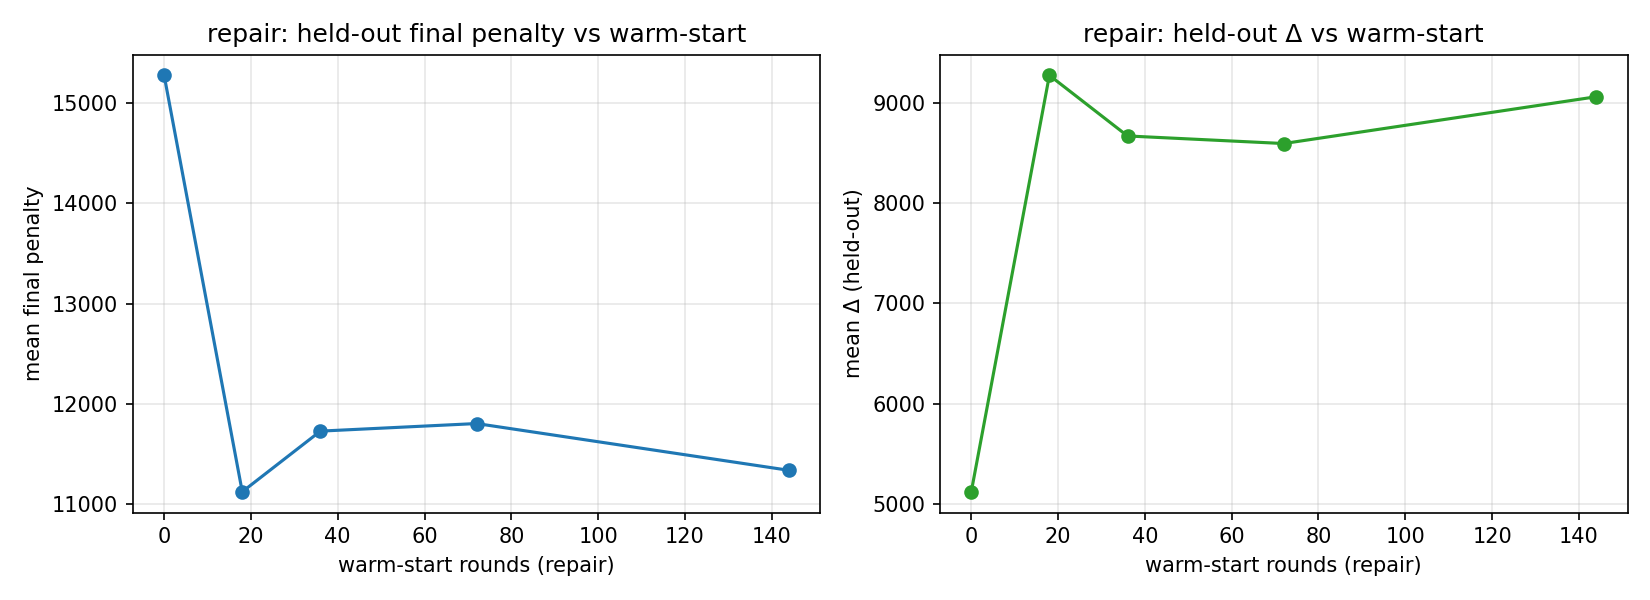
\includegraphics[width=0.48\textwidth]{experiment plots/experiment-05/warm_start_repair.png}
    \caption{Held-out dev mean final penalty and mean $\Delta$ vs.\ warm-start length at the week level (left) and repair level (right).}
    \label{fig:warm-start}
\end{figure}

\clearpage
\subsection{Training-set scaling} % Experiment - 06
\label{sec:data-scaling}
\begin{figure}[h]
    \centering
    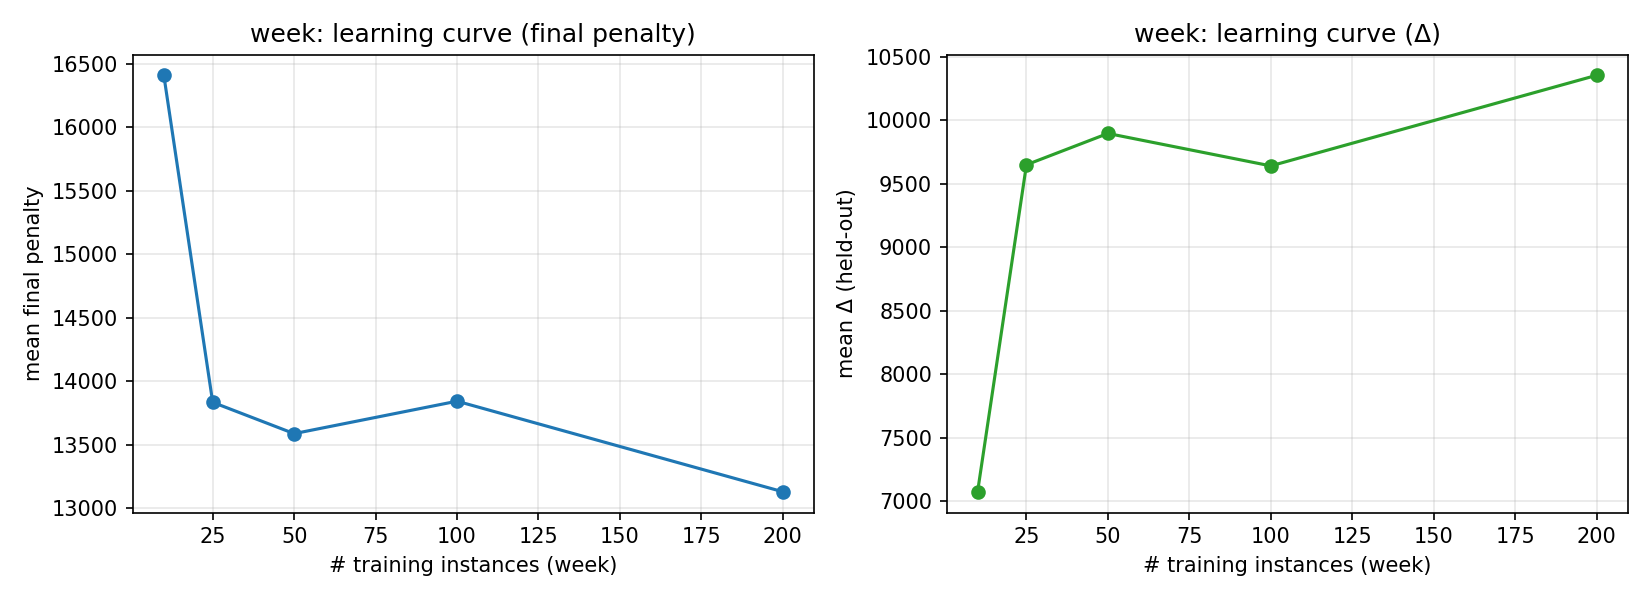
\includegraphics[width=0.48\textwidth]{experiment plots/experiment-06/data_scaling_week.png}
    \hfill
    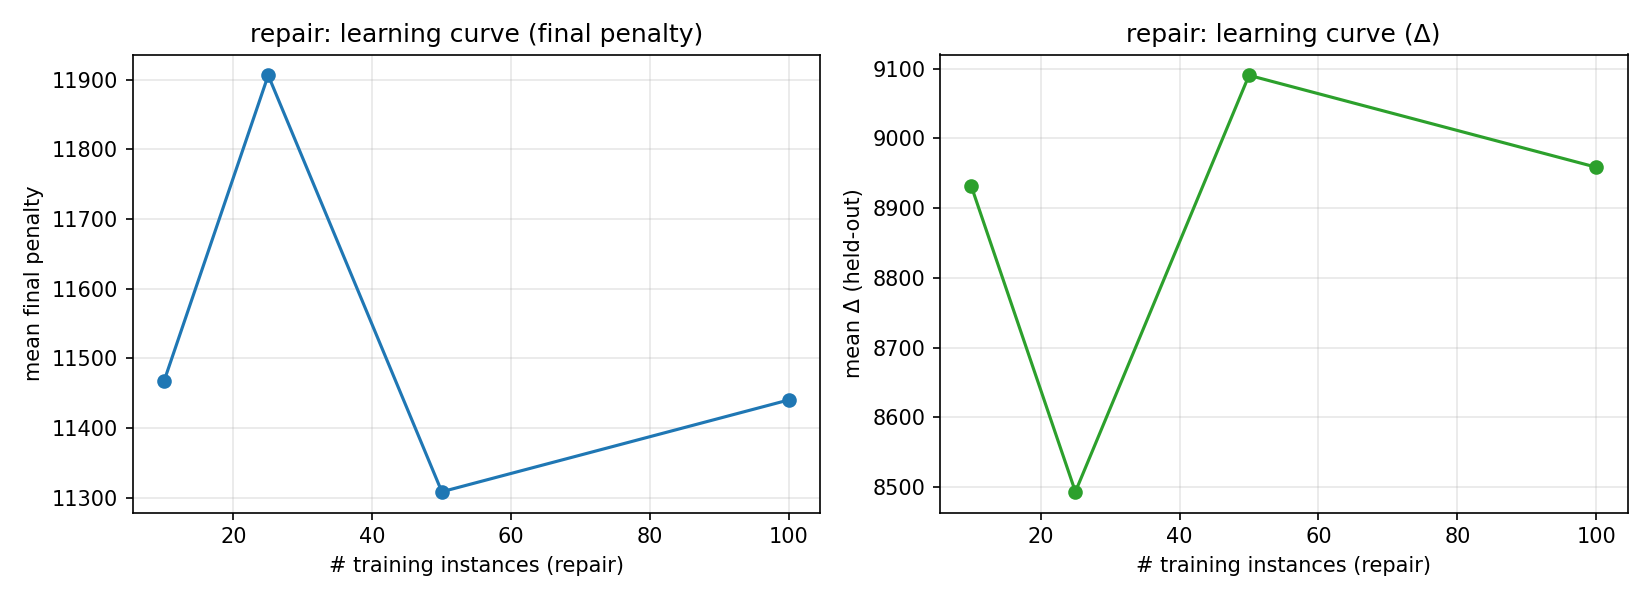
\includegraphics[width=0.48\textwidth]{experiment plots/experiment-06/data_scaling_repair.png}
    \caption{Held-out dev mean final penalty and mean $\Delta$ vs.\ number of training instances at the week level (left) and repair level (right).}
    \label{fig:data-scaling}
\end{figure}

Since a single $\hat{\theta}_a$ is shared across all training
scenarios, the training-set scaling experiment tests whether pooling
experience across more instances helps or hurts at each level. At the
week level, mean final penalty drops sharply with the first few
training instances and continues to decrease as the training set grows
to 200, indicating that the shared parameter estimate generalizes well
when the arm space is small and the context-to-action mapping is
smooth. At the repair level, however, performance is less stable with mean
final penalty gradually increases as training instances grow to 100,
suggesting that a single shared policy averages over instance-specific
operator dynamics that differ enough to make pooling counterproductive.
With 18 arms and schedule states that vary widely across scenarios, the
shared $\hat{\theta}_a$ appears to trade per-instance accuracy for
cross-instance generality in a regime where that trade-off is
unfavorable.

\subsection{Context ablation} % Experiment - 09
\label{sec:context-ablation}
\begin{figure}[h]
    \centering
    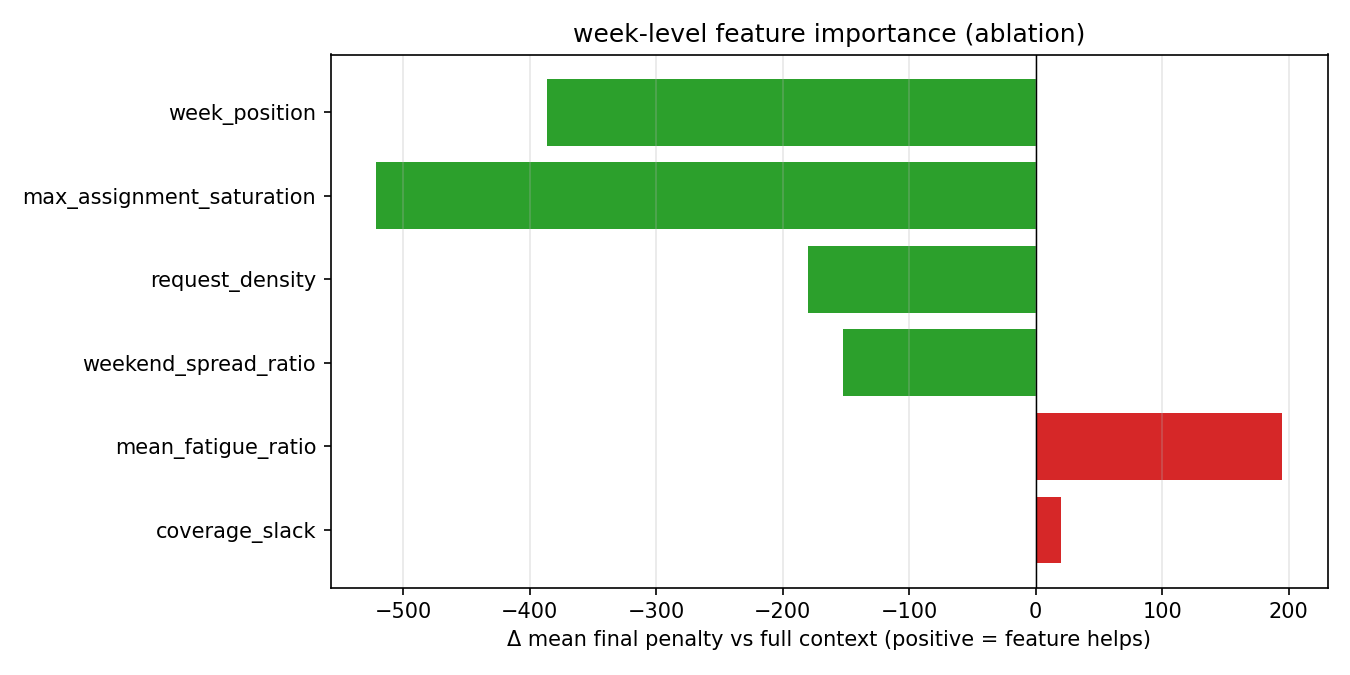
\includegraphics[width=0.48\textwidth]{experiment plots/experiment-09/ablation_week.png}
    \hfill
    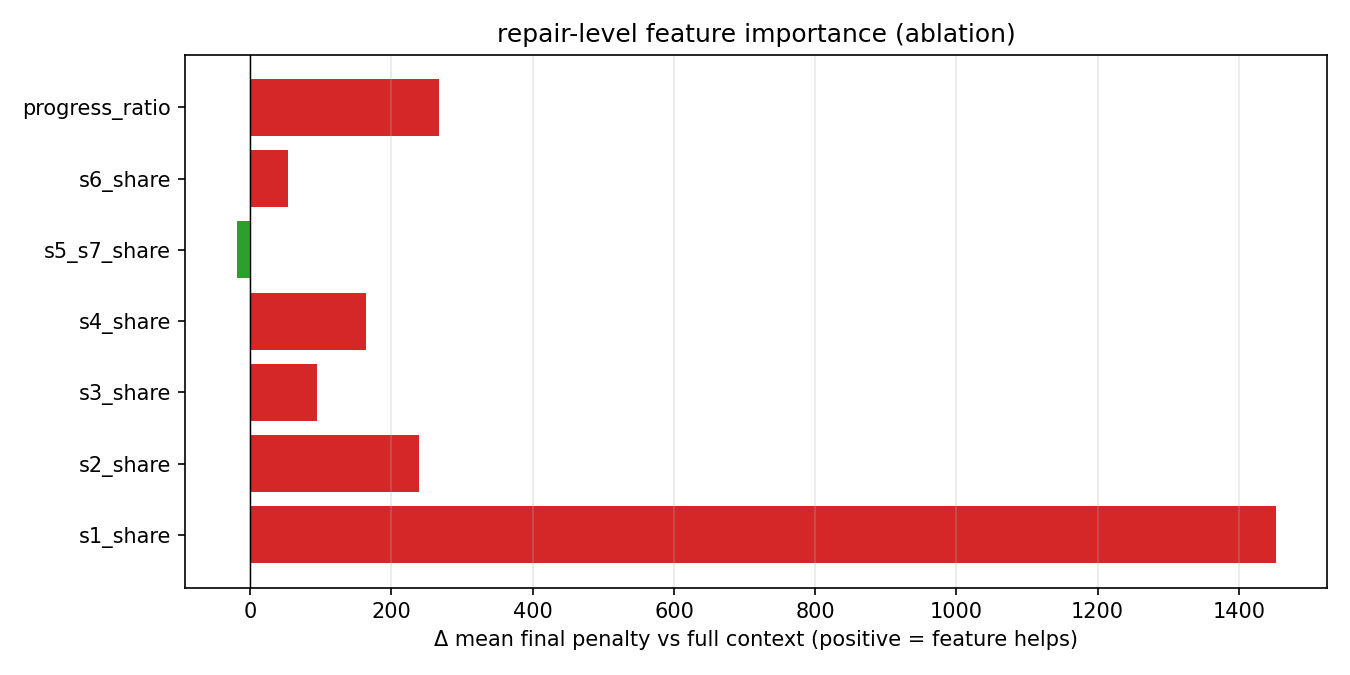
\includegraphics[width=0.48\textwidth]{experiment plots/experiment-09/ablation_repair.png}
    \caption{Context-feature ablation for the week-level bandit (left) and
    repair-level bandit (right). Each bar masks one feature while retraining
    LinUCB from scratch.}
    \label{fig:context-ablation}
\end{figure}

\subsection{Performance by instance size} % Experiment 10
\label{sec:size-breakdown}
\begin{figure}[h]
    \centering
    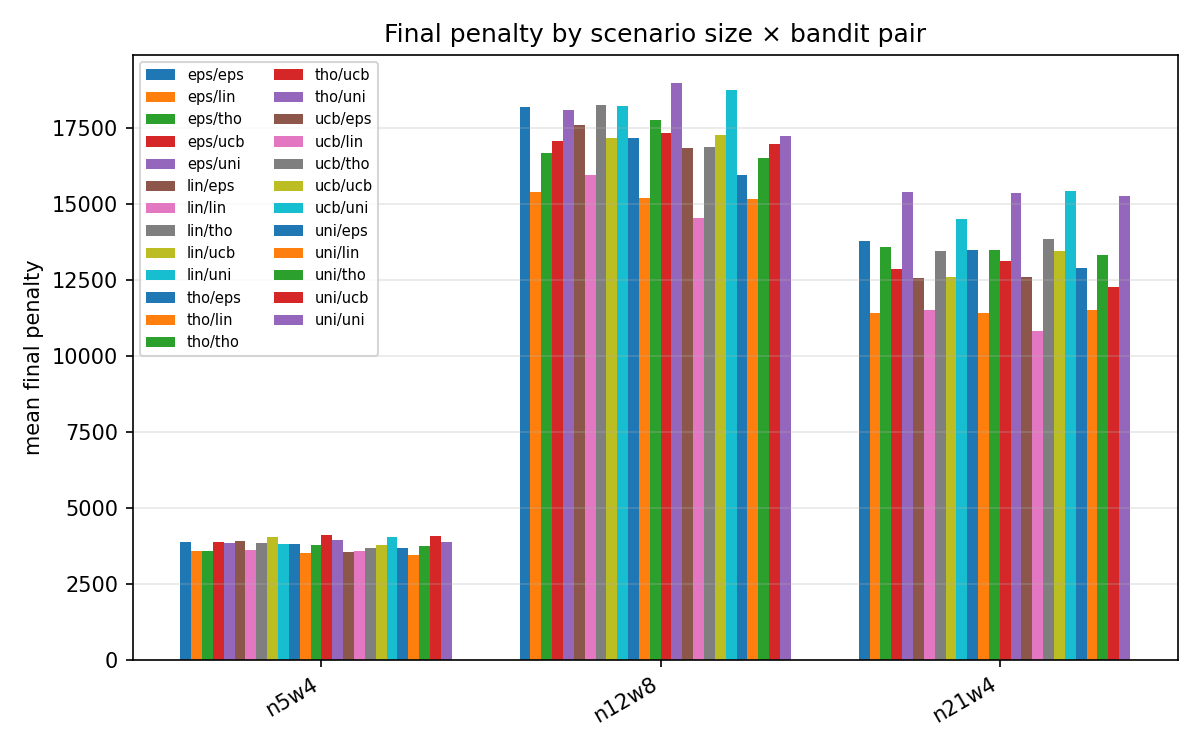
\includegraphics[width=0.48\textwidth]{experiment plots/experiment-10/size_bars.png}
    \hfill
    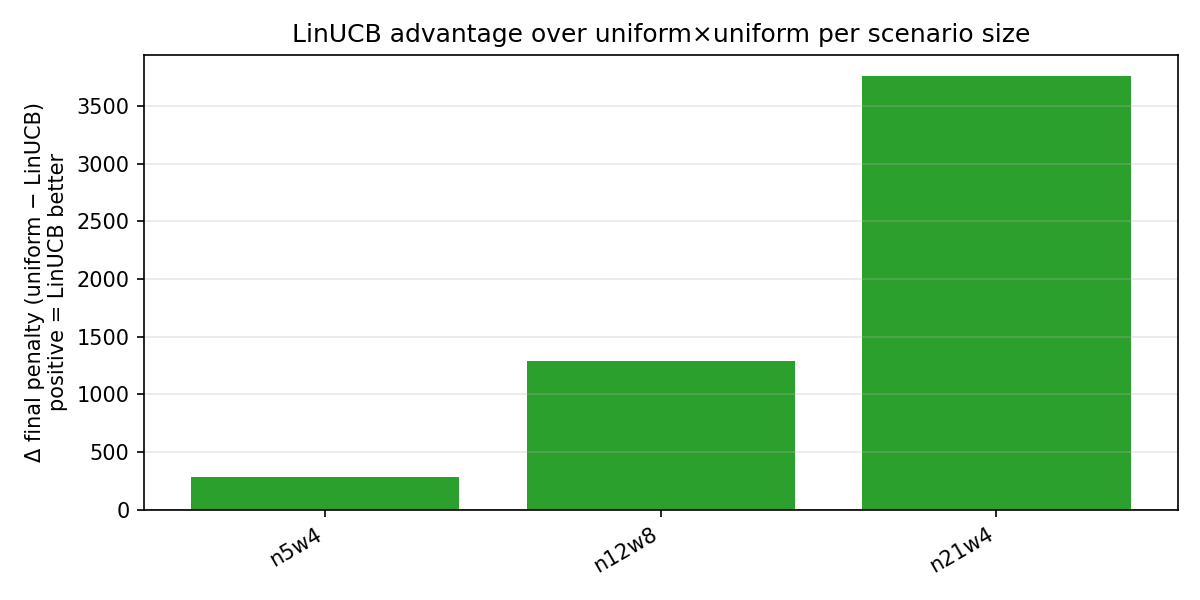
\includegraphics[width=0.48\textwidth]{experiment plots/experiment-10/linucb_advantage_by_size.png}
    \caption{Bandit performance by instance size. Left: mean final penalty
    by week-level and repair-level bandit pair. Right: average advantage of
    LinUCB repair over non-contextual repair methods by scenario size.}
    \label{fig:size-breakdown}
\end{figure}

\clearpage

\subsection{Out-of-distribution repair starts} % Experiment 11
\label{sec:ood-repair}

\begin{figure}[h]
    \centering
    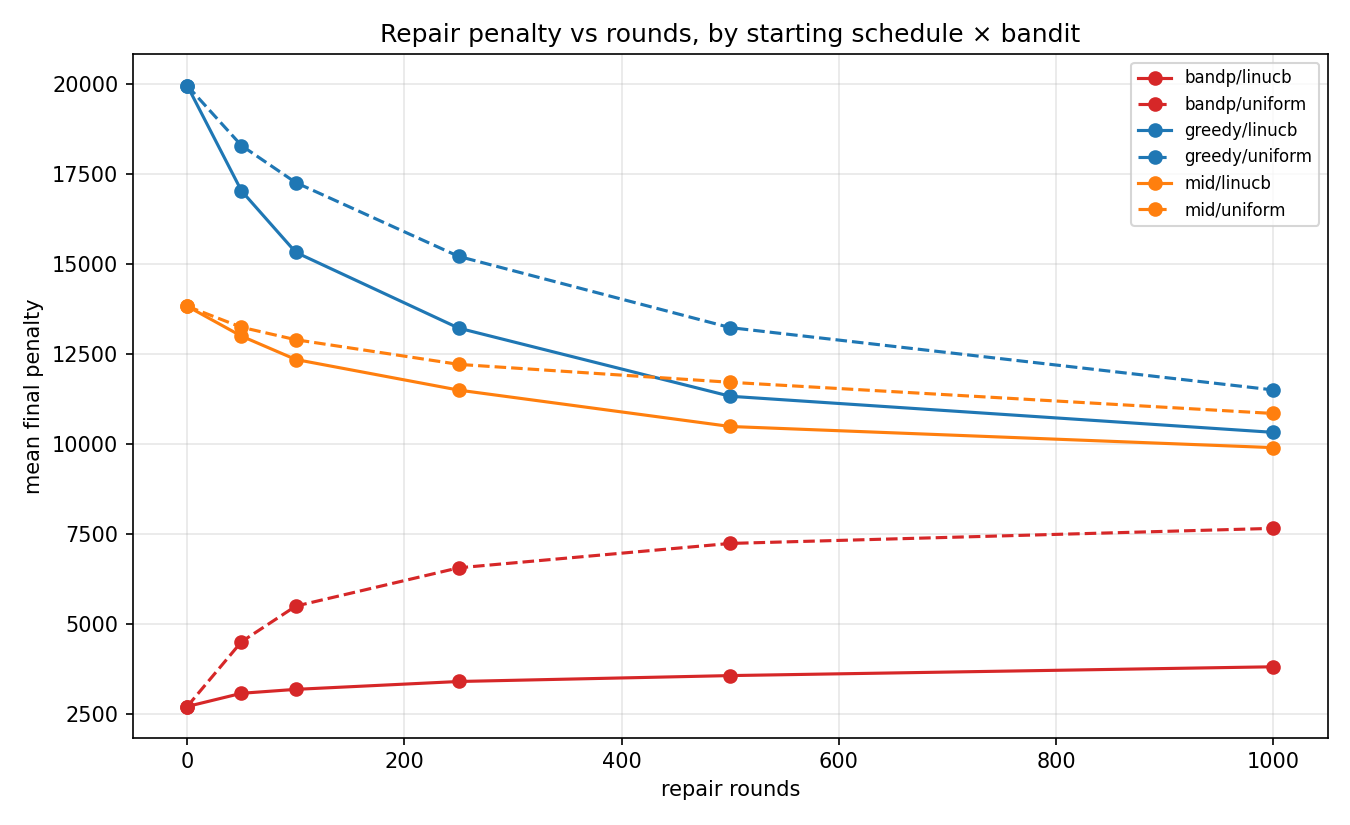
\includegraphics[width=0.48\textwidth]{experiment plots/experiment-11/ood_curves.png}
    \hfill
    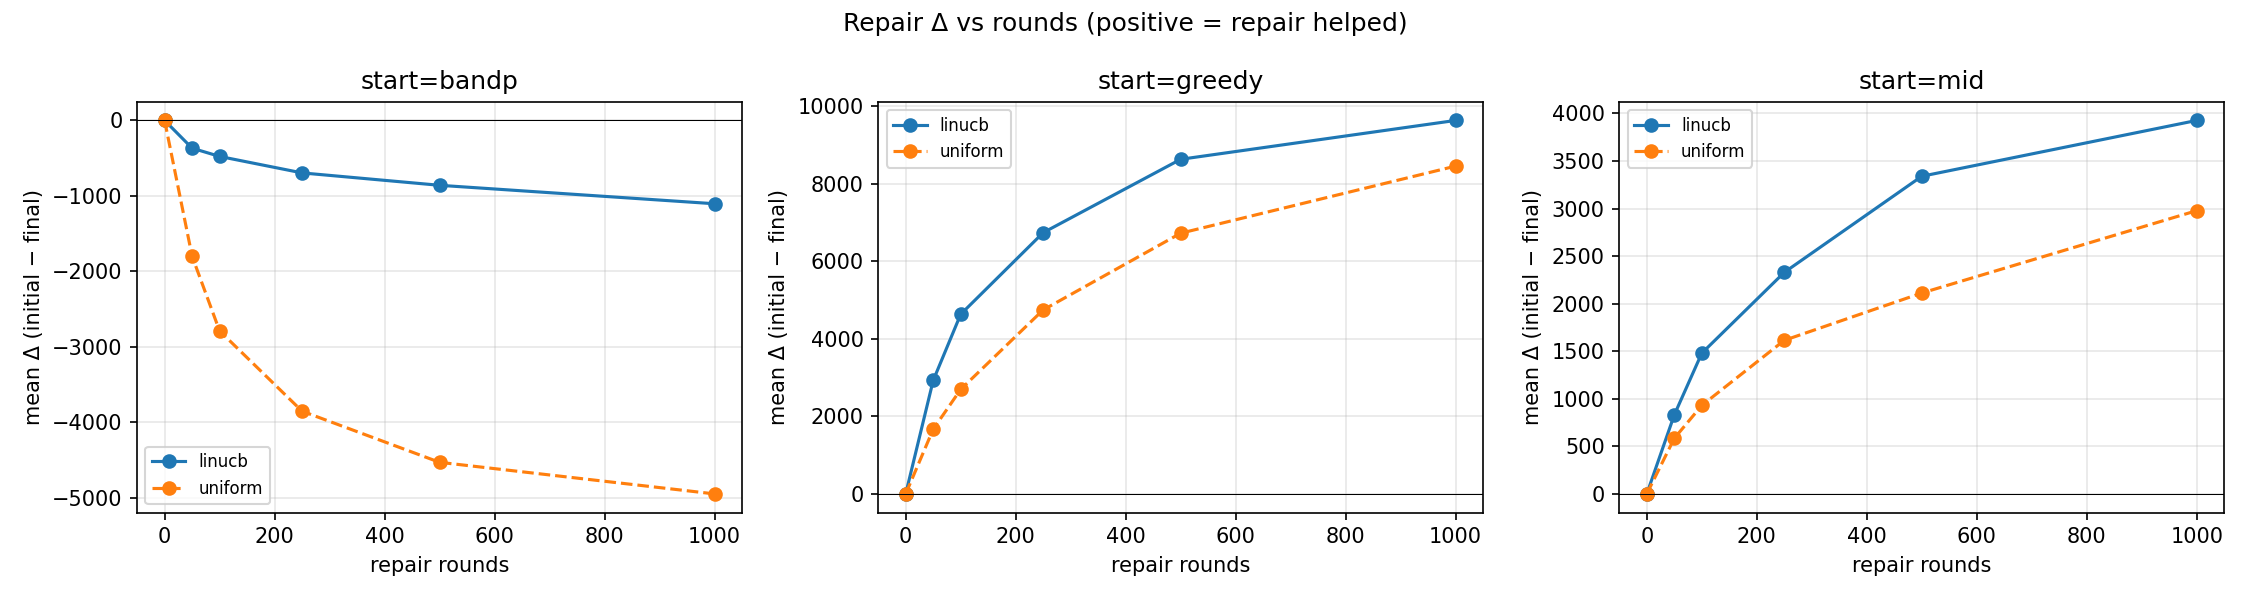
\includegraphics[width=0.48\textwidth]{experiment plots/experiment-11/ood_delta_per_start.png}
    \caption{Repair behavior under different starting-schedule
    distributions. LinUCB improves greedy and mid-quality starts, but
    degrades near-optimal branch-and-price starts.}
    \label{fig:ood-repair}
\end{figure}

\section{Open Problems and Future Directions}

\paragraph{Strengths and limitations of the bandit formulation}


The main theoretical strength is transparency as LinUCB provides a closed-form parameter estimate, an interpretable upper-confidence score per arm, and known regret scaling under its assumptions. This makes the pipeline easy to debug and cheap to train relative to deep RL. The main weakness is which Section 4.6 identifies — the regret bounds assume conditional independence of rewards given context, which fails at the repair level because the context vector is not a sufficient statistic for the schedule state. This means we have no formal performance guarantee for the repair bandit. A secondary weakness is that the week-level bandit operates over so few rounds per instance (4–8) that asymptotic regret bounds are uninformative regardless of whether assumptions hold. Our empirical results are the only evidence that the method works, and they are limited to the INRC-II benchmark.

\paragraph{From bandit to MDP.}
Our central negative result — that the repair bandit degrades
near-optimal schedules (Experiment~11) — is evidence that the problem
has sequential structure the bandit formulation discards. The repair
reward at round $j$ depends on the full action history through its
effect on the schedule, a dependency that a Markov decision process
captures but a bandit does not. The natural question is whether an MDP
formulation, where the state is the schedule and the action is a repair
operator, recovers the lost value, and at what computational cost. Our
OOD experiment provides a lower bound on the value of sequential
reasoning: the gap between LinUCB repair and no repair at all on
branch-and-price schedules. Whether an MDP policy can close this gap,
and whether the additional sample complexity is justified for schedules
that are already near-optimal, remains open. A lightweight intermediate
step would be to allow online LinUCB updates during inference —
continuing to accumulate $(A_a, b_a)$ on the fly — though it is unclear
whether the bandit can adapt fast enough within a single instance's 500
repair rounds for this to help.

\paragraph{Instance-size invariance of the repair context.}
The repair context maps penalty contributions onto a probability simplex
so that the bandit conditions on which constraint dominates rather than
on absolute penalty magnitude (Section~4.4). This design assumes that
the relative penalty profile is a sufficient statistic for choosing
repair actions regardless of instance size. Experiment~10 shows that
LinUCB's advantage over non-contextual methods varies across scenario
sizes, but does not isolate whether this variation reflects a failure of
the invariance assumption or differences in problem structure. A
controlled cross-size transfer experiment — training on one size bracket
and evaluating on another — would test whether the normalized context
transfers across scales or whether size-specific features are needed.

\paragraph{Additional experiments not yet performed.}
Several experiments would strengthen the empirical case but were not
completed within the project timeline. First, a per-arm selection
frequency analysis showing how LinUCB's arm choices vary across context
regimes would confirm that the contextual policy learns a differentiated
strategy rather than collapsing to a dominant arm. Second, cumulative
regret curves against the best-fixed-arm oracle would quantify learning
speed and connect the empirical results to the theoretical regret
discussion in Section~4.6. Third, the cross-size transfer experiment
described above would directly test the repair context's invariance
property. These were deferred because the primary experimental effort
focused on establishing the algorithm comparison and identifying the
regime of applicability, which we judged to be the more fundamental
contribution.
--------------------------